% datastruct/datastruct.tex

\QuickQuizChapter{chp:Data Structures}{Data Structures}

Efficient access to data is critically important to performance, and
therefore discussions of algorithms therefore focus heavily on the
time complexity of the related
data structures~\cite{ThomasHCorman2001Algorithms}.
However, for parallel programs, measures of time complexity must also
include the effects of concurrency.
These concurrency effects can be overwhelmingly large, as discussed in
Chapter~\ref{chp:Hardware and its Habits}, which means that design of
concurrent data structures must pay at least as much attention to the
concurrency effects as it does to the classical sequential time
complexity.

Section~\ref{sec:datastruct:Motivating Application}
presents a motivating application that will be used to evaluate
the data structures presented in this chapter.

As discussed in Chapter~\ref{cha:Partitioning and Synchronization Design},
an excellent way to achieve high scalability is partitioning.
This points the way to partitionable data structures, a topic taken up by
Section~\ref{sec:datastruct:Partitionable Data Structures}.
Chapter~\ref{chp:Deferred Processing} described how deferring some
actions can greatly improve both performance and scalability.
Section~\ref{sec:defer:Read-Copy Update (RCU)} in particular showed
how to tap the awesome power of procrastination in pursuit of
performance and scalability, a topic taken up by
Section~\ref{sec:datastruct:Read-Mostly Data Structures}.

Not all data structures are partitionable.
Section~\ref{sec:datastruct:Non-Partitionable Data Structures}
looks at a mildly non-partitionable example data structure.
This section shows
how to split it into read-mostly and partitionable portions,
enabling a fast and scalable implementation.

Because this chapter cannot delve into the details of every concurrent
data structure that has ever been used
Section~\ref{sec:datastruct:Other Data Structures}
provides a brief survey of the most common and important ones.
Although the best performance and scalability results design rather
than after-the-fact micro-optimization, it is nevertheless the case
that micro-optimization has an important place in achieving the
absolute best possible performance and scalability.
This topic is therefore taken up in
Section~\ref{sec:datastruct:Micro-Optimization}.

Finally, Section~\ref{sec:datastruct:Summary}
presents a summary of this chapter.

\section{Motivating Application}
\label{sec:datastruct:Motivating Application}

We will use the Schr\"odinger's Zoo application to evaluate
performance~\cite{McKenney:2013:SDS:2483852.2483867}.
Schr\"odinger has a zoo containing a large number of animals, and
he would like to track them using an in-memory database with
each animal in the zoo represented by a data item in this database.
Each animal has a unique name that is used as a key, with a variety
of data tracked for each animal.

Births, captures, and purchases result in insertions, while deaths,
releases, and sales result in deletions.
Because Schr\"odinger's zoo contains a large quantity of short-lived
animals, including mice and insects, the database must be able to
support a high transaction rate.

Those interested in Schr\"odinger's animals can query them, however,
Schr\"odinger has noted an extremely high rate of queries for his cat,
so much so that he suspects that his mice might be using the database
to check up on their nemesis.
This means that Sch\"odinger's application must be able to support a
high rate of queries to a single data element.

Please keep this application in mind as various data structures are presented.

\section{Partitionable Data Structures}
\label{sec:datastruct:Partitionable Data Structures}

There are a huge number of data structures in use today, so much so
that there are multiple textbooks covering them.
Given that this section is intended to be smaller than a full textbook,
it will focus on a single data structure, namely the hash table.
This approach allows a much deeper investigation of how concurrency
interacts with data structures, and also focuses on a data structure
that is heavily used in practice.
Section~\ref{sec:datastruct:Non-Partitionable Data Structures}
touches on non-partitionable data structures in
the form of a resizable hash table, and
Section~\ref{sec:datastruct:Other Data Structures}
gives a brief review of other concurrent data structures.

\subsection{Hash-Table Design}
\label{sec:datastruct:Hash-Table Design}

Chapter~\ref{cha:Partitioning and Synchronization Design}
emphasized the need to apply partitioning in order to attain
respectable performance and scalability, so partitionability
must be a first-class criterion when selecting data structures.
This criterion is well satisfied by that workhorse of parallelism,
the hash table.
Hash tables are conceptually simple, consisting of an array of
\emph{hash buckets}.
A \emph{hash function} maps from a given element's \emph{key}
to the hash bucket that this element will be stored in.
Each hash bucket therefore heads up a linked list of elements,
called a \emph{hash chain}.
When properly configured, these hash chains will be quite short,
permitting a hash table to access the element with a given key
extremely efficiently.

\QuickQuiz{}
	But there are many types of hash tables, of which the chained
	hash tables described here are but one type.
	Why the focus on chained hash tables?
\QuickQuizAnswer{
	Chained hash tables are completely partitionable, and thus
	well-suited to concurrent use.
	There are other completely-partitionable hash tables, for
	example, split-ordered list~\cite{OriShalev2006SplitOrderListHash},
	but they are considerably more complex.
	We therefore start with chained hash tables.
} \QuickQuizEnd

In addition, each bucket can be given its own lock, so that
elements in different buckets of the hash table may be added,
deleted, and looked up completely independently.
A large hash table containing a large number of elements therefore
offers excellent scalability.

\subsection{Hash-Table Implementation}
\label{sec:datastruct:Hash-Table Implementation}

\begin{figure}[tb]
{ \scriptsize
\begin{verbatim}
 1 struct ht_elem {
 2   struct cds_list_head hte_next;
 3   unsigned long hte_hash;
 4 };
 5 
 6 struct ht_bucket {
 7   struct cds_list_head htb_head;
 8   spinlock_t htb_lock;
 9 };
10 
11 struct hashtab {
12   unsigned long ht_nbuckets;
13   struct ht_bucket ht_bkt[0];
14 };
\end{verbatim}
}
\caption{Hash-Table Data Structures}
\label{fig:datastruct:Hash-Table Data Structures}
\end{figure}

\begin{figure}[tb]
\begin{center}
\resizebox{3in}{!}{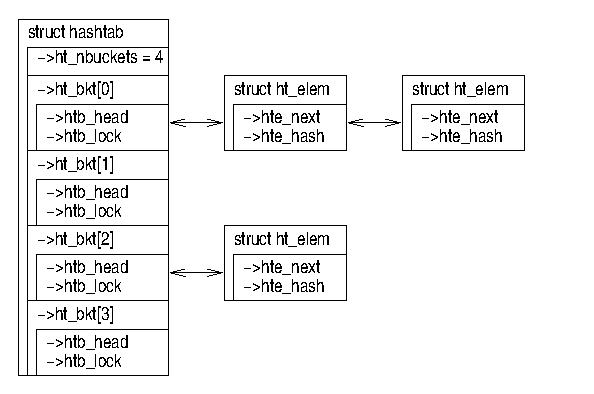
\includegraphics{datastruct/hashdiagram}}
\end{center}
\caption{Hash-Table Data-Structure Diagram}
\label{fig:datastruct:Hash-Table Data-Structure Diagram}
\end{figure}

Figure~\ref{fig:datastruct:Hash-Table Data Structures}
(\co{hash_bkt.c})
shows a set of data structures used in a simple fixed-sized hash
table using chaining and per-hash-bucket locking, and
Figure~\ref{fig:datastruct:Hash-Table Data-Structure Diagram}
diagrams how they fit together.
The \co{hashtab} structure (lines~11-14 in
Figure~\ref{fig:datastruct:Hash-Table Data Structures})
contains four \co{ht_bucket} structures (lines~6-9
Figure~\ref{fig:datastruct:Hash-Table Data Structures}),
with the \co{->bt_nbuckets} field controlling the number of buckets.
Each such bucket contains a list header \co{->htb_head} and
a lock \co{->htb_lock}.
The list headers chain \co{ht_elem} structures
(lines~1-4 in
Figure~\ref{fig:datastruct:Hash-Table Data Structures})
through their
\co{->hte_next} fields, and each \co{ht_elem} structure also caches
the corresponding element's hash value in the \co{->hte_hash} field.
The \co{ht_elem} structure would be included in the larger structure
being placed in the hash table, and this larger structure might contain
a complex key.

The diagram shown in
Figure~\ref{fig:datastruct:Hash-Table Data-Structure Diagram}
has bucket~0 with two elements and bucket~2 with one.

\begin{figure}[tb]
{ \scriptsize
\begin{verbatim}
 1 #define HASH2BKT(htp, h) \
 2   (&(htp)->ht_bkt[h % (htp)->ht_nbuckets])
 3 
 4 static void hashtab_lock(struct hashtab *htp,
 5                          unsigned long hash)
 6 {
 7   spin_lock(&HASH2BKT(htp, hash)->htb_lock);
 8 }
 9 
10 static void hashtab_unlock(struct hashtab *htp,
11                            unsigned long hash)
12 {
13   spin_unlock(&HASH2BKT(htp, hash)->htb_lock);
14 }
\end{verbatim}
}
\caption{Hash-Table Mapping and Locking}
\label{fig:datastruct:Hash-Table Mapping and Locking}
\end{figure}

Figure~\ref{fig:datastruct:Hash-Table Mapping and Locking}
shows mapping and locking functions.
Lines~1 and~2 show the macro \co{HASH2BKT()}, which maps from a hash value
to the corresponding \co{ht_bucket} structure.
This macro uses a simple modulus: if more aggressive hashing is required,
the caller needs to implement it when mapping from key to hash value.
The remaining two functions acquire and release the \co{->htb_lock}
corresponding to the specified hash value.

\begin{figure}[tb]
{ \scriptsize
\begin{verbatim}
 1 struct ht_elem *
 2 hashtab_lookup(struct hashtab *htp,
 3                unsigned long hash,
 4                void *key,
 5                int (*cmp)(struct ht_elem *htep,
 6                           void *key))
 7 {
 8   struct ht_bucket *htb;
 9   struct ht_elem *htep;
10 
11   htb = HASH2BKT(htp, hash);
12   cds_list_for_each_entry(htep,
13                           &htb->htb_head,
14                           hte_next) {
15     if (htep->hte_hash != hash)
16       continue;
17     if (cmp(htep, key))
18       return htep;
19   }
20   return NULL;
21 }
\end{verbatim}
}
\caption{Hash-Table Lookup}
\label{fig:datastruct:Hash-Table Lookup}
\end{figure}

Figure~\ref{fig:datastruct:Hash-Table Lookup}
shows \co{hashtab_lookup()},
which returns a pointer to the element with the specified hash and key if it
exists, or \co{NULL} otherwise.
This function takes both a hash value and a pointer to the key because
this allows users of this function to use arbitrary keys and
arbitrary hash functions, with the key-comparison function passed in via
\co{cmp()}, in a manner similar to \co{qsort()}.
Line~11 maps from the hash value to a pointer to the corresponding
hash bucket.
Each pass through the loop spanning line~12-19 examines one element
of the bucket's hash chain.
Line~15 checks to see if the hash values match, and if not, line~16
proceeds to the next element.
Line~17 checks to see if the actual key matches, and if so,
line~18 returns a pointer to the matching element.
If no element matches, line~20 returns \co{NULL}.

\QuickQuiz{}
	But isn't the double comparison on lines~15-18 in
	Figure~\ref{fig:datastruct:Hash-Table Lookup} inefficient
	in the case where the key fits into an unsigned long?
\QuickQuizAnswer{
	Indeed it is!
	However, hash tables quite frequently store information with
	keys such as character strings that do not necessarily fit
	into an unsigned long.
	Simplifying the hash-table implementation for the case where
	keys always fit into unsigned longs is left as an exercise
	for the reader.
} \QuickQuizEnd

\begin{figure}[tb]
{ \scriptsize
\begin{verbatim}
 1 void
 2 hashtab_add(struct hashtab *htp,
 3             unsigned long hash,
 4             struct ht_elem *htep)
 5 {
 6   htep->hte_hash = hash;
 7   cds_list_add(&htep->hte_next,
 8                &HASH2BKT(htp, hash)->htb_head);
 9 }
10 
11 void hashtab_del(struct ht_elem *htep)
12 {
13   cds_list_del_init(&htep->hte_next);
14 }
\end{verbatim}
}
\caption{Hash-Table Modification}
\label{fig:datastruct:Hash-Table Modification}
\end{figure}

Figure~\ref{fig:datastruct:Hash-Table Modification}
shows the \co{hashtab_add()} and \co{hashtab_del()} functions
that add and delete elements from the hash table, respectively.

The \co{hashtab_add()} function simply sets the element's hash
value on line~6, then adds it to the corresponding bucket on
lines~7 and~8.
The \co{hashtab_del()} function simply removes the specified element
from whatever hash chain it is on, courtesy of the doubly linked
nature of the hash-chain lists.
Before calling either of these two functions, the caller is required to
ensure that no other thread is accessing
or modifying this same bucket, for example, by invoking
\co{hashtab_lock()} beforehand.

\begin{figure}[tb]
{ \scriptsize
\begin{verbatim}
 1 struct hashtab *
 2 hashtab_alloc(unsigned long nbuckets)
 3 {
 4   struct hashtab *htp;
 5   int i;
 6 
 7   htp = malloc(sizeof(*htp) +
 8                nbuckets *
 9                sizeof(struct ht_bucket));
10   if (htp == NULL)
11     return NULL;
12   htp->ht_nbuckets = nbuckets;
13   for (i = 0; i < nbuckets; i++) {
14     CDS_INIT_LIST_HEAD(&htp->ht_bkt[i].htb_head);
15     spin_lock_init(&htp->ht_bkt[i].htb_lock);
16   }
17   return htp;
18 }
19 
20 void hashtab_free(struct hashtab *htp)
21 {
22   free(htp);
23 }
\end{verbatim}
}
\caption{Hash-Table Allocation and Free}
\label{fig:datastruct:Hash-Table Allocation and Free}
\end{figure}

Figure~\ref{fig:datastruct:Hash-Table Allocation and Free}
shows \co{hashtab_alloc()} and \co{hashtab_free()},
which do hash-table allocation and freeing, respectively.
Allocation begins on lines~7-9 with allocation of the underlying memory.
If line~10 detects that memory has been exhausted, line~11 returns
\co{NULL} to the caller.
Otherwise, line~11 initializes the number of buckets, and the loop
spanning lines~13-16 initializes the buckets themselves,
including the chain list header on line~14 and the lock on line~15.
Finally, line~17 returns a pointer to the newly allocated hash table.
The \co{hashtab_free()} function on lines~20-23 is straightforward.

\subsection{Hash-Table Performance}
\label{sec:datastruct:Hash-Table Performance}

\begin{figure}[tb]
\begin{center}
\resizebox{3in}{!}{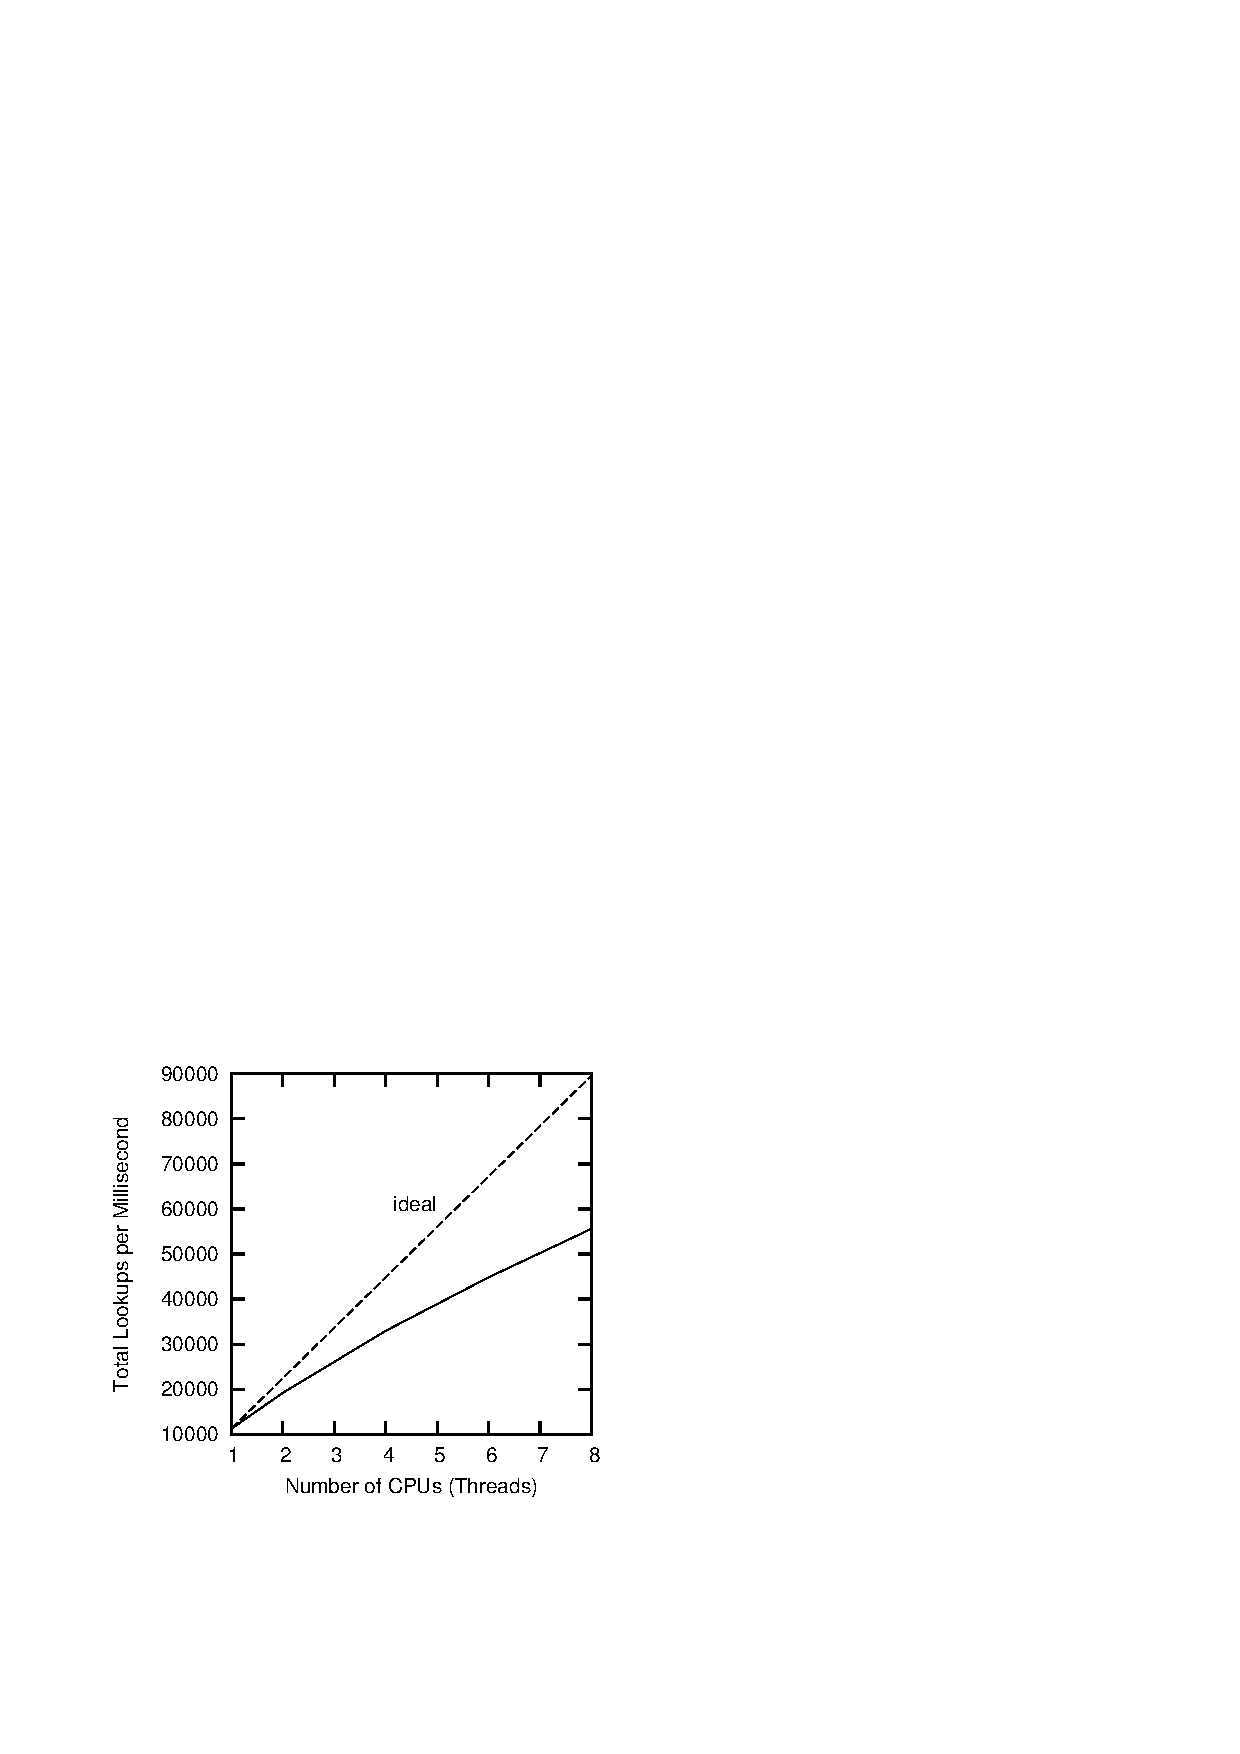
\includegraphics{datastruct/zoocpubktlin8}}
\end{center}
\caption{Read-Only Hash-Table Performance For Schr\"odinger's Zoo}
\label{fig:datastruct:Read-Only Hash-Table Performance For Schroedinger's Zoo}
\end{figure}

The performance results for an eight-CPU 2GHz
Intel\textsuperscript\textregistered
Xeon\textsuperscript\textregistered
system using a bucket-locked hash table with 1024 buckets are shown in
Figure~\ref{fig:datastruct:Read-Only Hash-Table Performance For Schroedinger's Zoo}.
The performance does scale nearly linearly, but is not much more than half
of the ideal performance level, even at only eight CPUs.
Part of this shortfall is due to the fact that the lock acquisitions and
releases incur no cache misses on a single CPU, but do incur misses
on two or more CPUs.

\begin{figure}[tb]
\begin{center}
\resizebox{3in}{!}{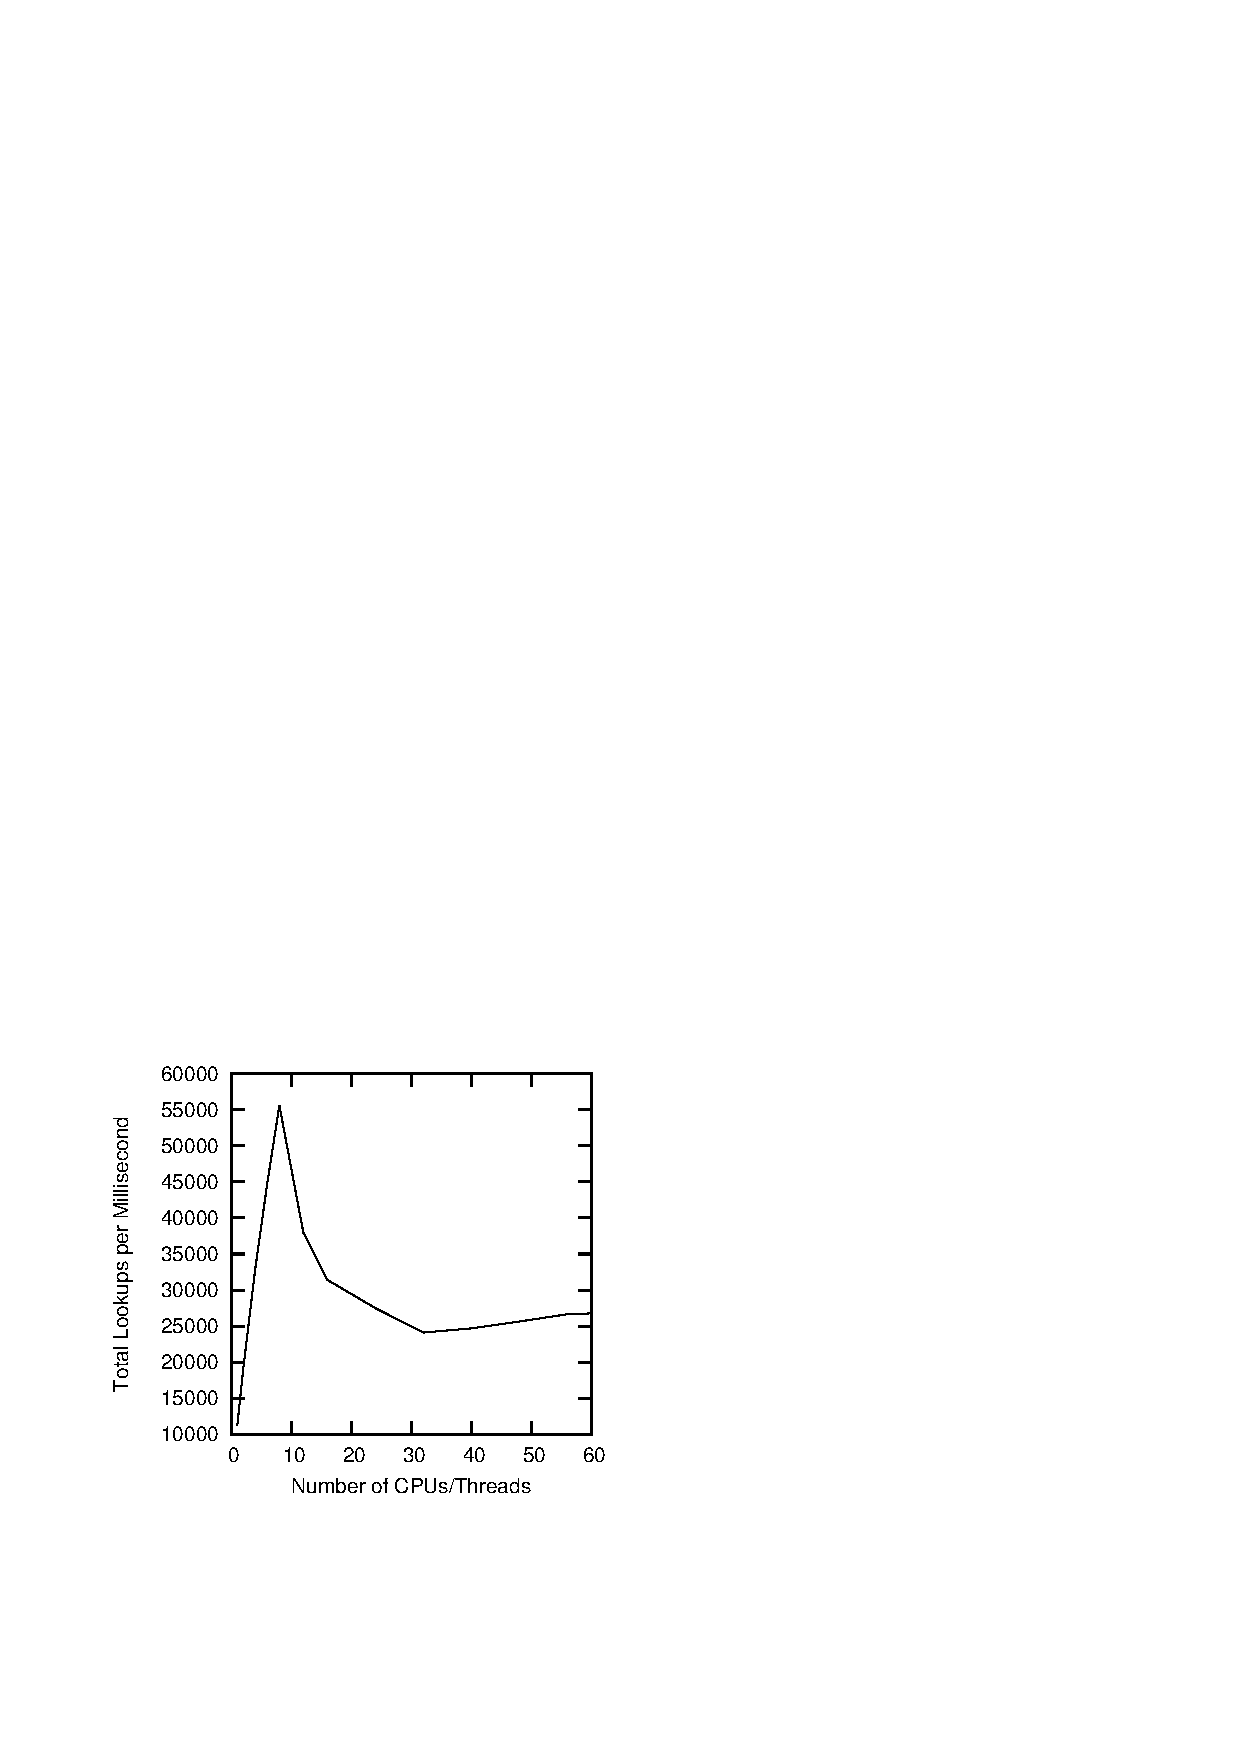
\includegraphics{datastruct/zoocpubktlin}}
\end{center}
\caption{Read-Only Hash-Table Performance For Schr\"odinger's Zoo, 60 CPUs}
\label{fig:datastruct:Read-Only Hash-Table Performance For Schroedinger's Zoo, 60 CPUs}
\end{figure}

And things only get worse with larger number of CPUs, as can be seen in
Figure~\ref{fig:datastruct:Read-Only Hash-Table Performance For Schroedinger's Zoo, 60 CPUs}.
We do not need an additional line to show ideal performance: The performance
for nine CPUs and beyond is worse than abysmal.
This clearly underscores the dangers of extrapolating performance from a
modest number of CPUs.

Of course, one possible reason for the collapse in performance might be
that more hash buckets are needed.
After all, we did not pad each hash bucket to a full cache line, so
there are a number of hash buckets per cache line.
It is possible that the resulting cache-thrashing comes into play at
nine CPUs.
This is of course easy to test by increasing the number of hash buckets.

\begin{figure}[tb]
\begin{center}
\resizebox{3in}{!}{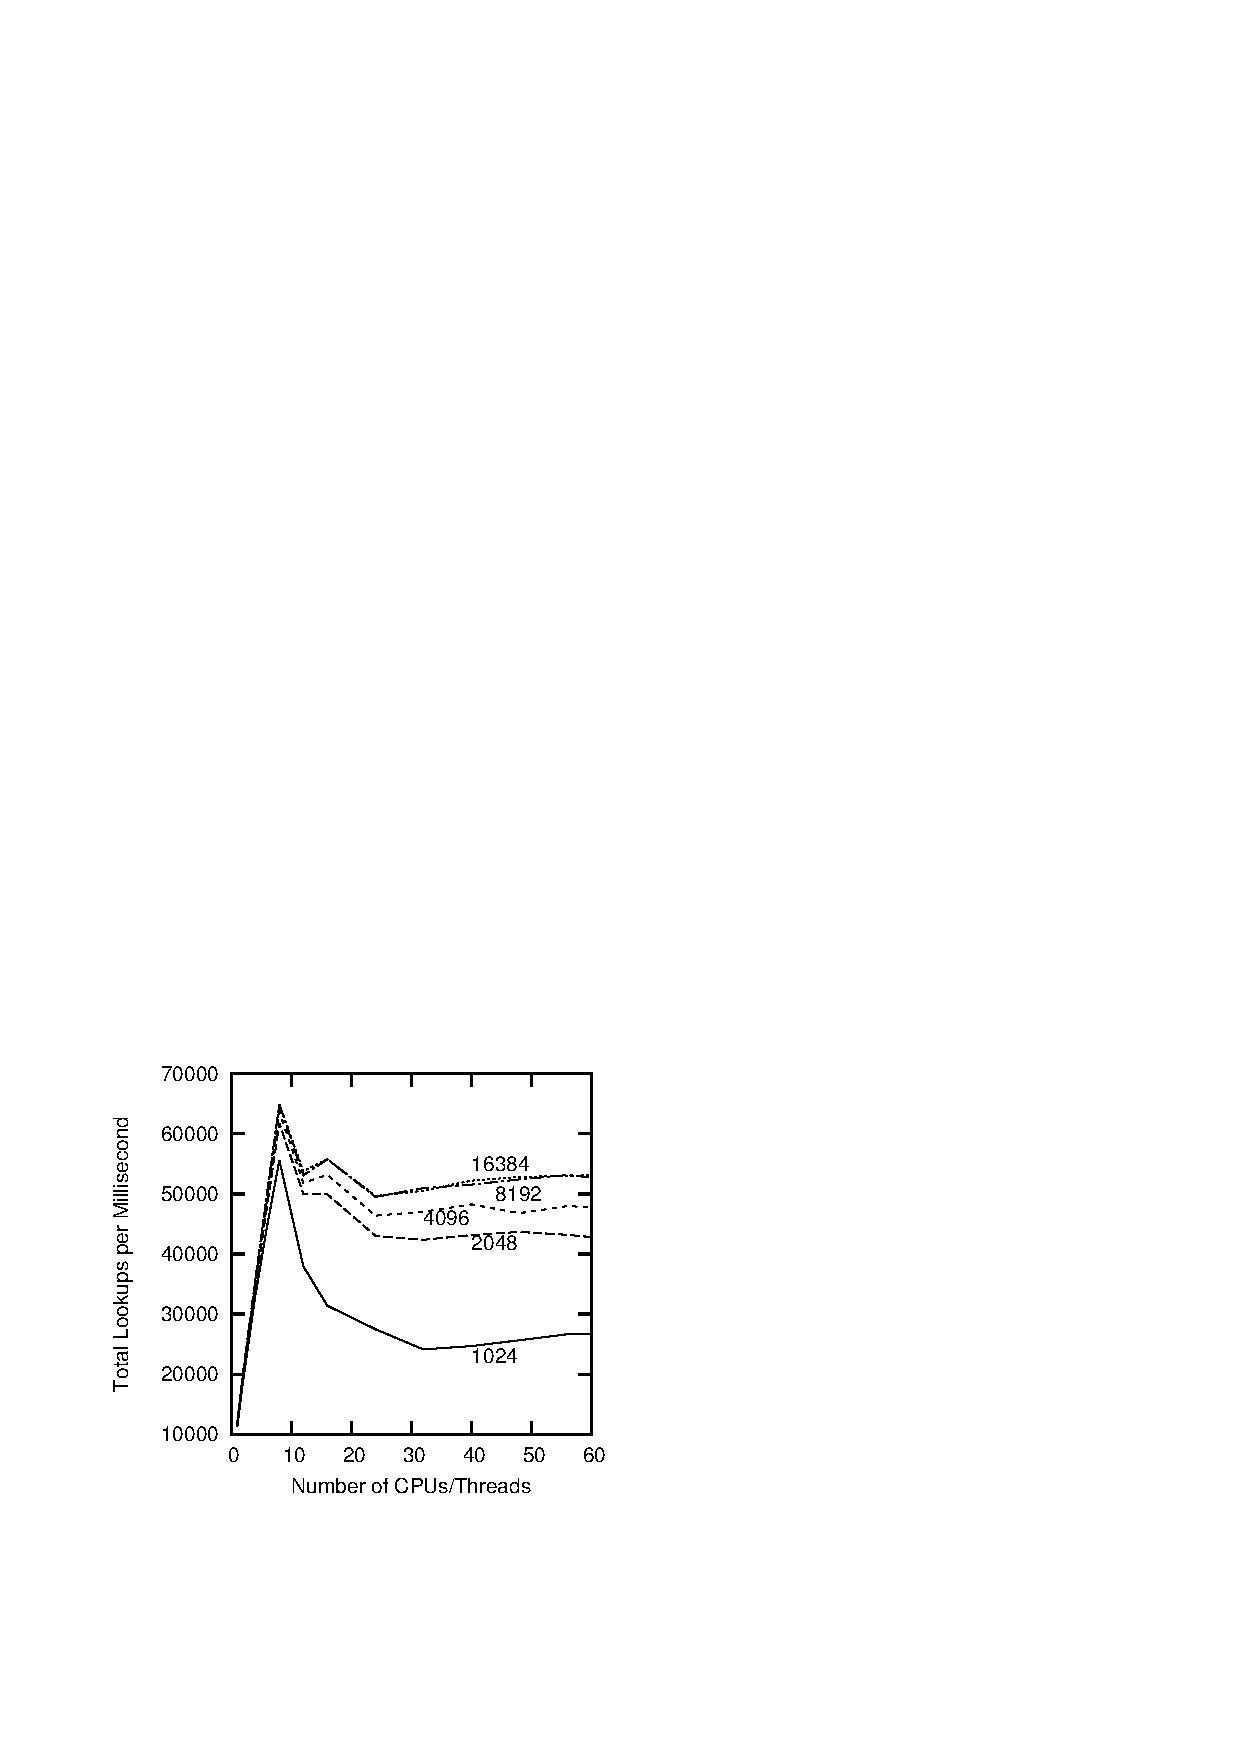
\includegraphics{datastruct/zoocpubktsizelin}}
\end{center}
\caption{Read-Only Hash-Table Performance For Schr\"odinger's Zoo, Varying Buckets}
\label{fig:datastruct:Read-Only Hash-Table Performance For Schroedinger's Zoo, Varying Buckets}
\end{figure}

However, as can be seen in
Figure~\ref{fig:datastruct:Read-Only Hash-Table Performance For Schroedinger's Zoo, Varying Buckets},
although increasing the number of buckets does increase performance somewhat,
scalability is still abysmal.
In particular, we still see a sharp dropoff at nine CPUs and beyond.
Furthermore, going from 8192 buckets to 16,384 buckets produced almost
no increase in performance.
Clearly something else is going on.

\begin{table}
\begin{center}
\begin{tabular}{r|r|r|r|r|r|r|r|r}
	Socket & \multicolumn{8}{|c}{Core} \\
	\hline
	0 &  0 &  1 &  2 &  3 &  4 &  5 &  6 &  7 \\
	  & 32 & 33 & 34 & 35 & 36 & 37 & 38 & 39 \\
	\hline
	1 &  8 &  9 & 10 & 11 & 12 & 13 & 14 & 15 \\
	  & 40 & 41 & 42 & 43 & 44 & 45 & 46 & 47 \\
	\hline
	2 & 16 & 17 & 18 & 19 & 20 & 21 & 22 & 23 \\
	  & 48 & 49 & 50 & 51 & 52 & 53 & 54 & 55 \\
	\hline
	3 & 24 & 25 & 26 & 27 & 28 & 29 & 30 & 31 \\
	  & 56 & 47 & 58 & 59 & 60 & 61 & 62 & 63 \\
\end{tabular}
\end{center}
\caption{NUMA Topology of System Under Test}
\label{tab:datastruct:NUMA Topology of System Under Test}
\end{table}

The problem is that this is a multi-socket system, with CPUs~0-7
and~32-39 mapped to the first socket as shown in
Table~\ref{tab:datastruct:NUMA Topology of System Under Test}.
Test runs confined to the first eight CPUs therefore perform quite
well, but tests that involve socket~0's CPUs~0-7 as well as
socket~1's CPU~8 incur the overhead of passing data across
socket boundaries.
This can severely degrade performance, as was discussed in
Section~\ref{sec:cpu:Hardware System Architecture}.

\QuickQuiz{}
	Given the negative scalability of the Schr\"odinger's
	Zoo application across sockets, why not just run multiple
	copies of the application, with each copy having a subset
	of the animals and confined to run on a single socket?
\QuickQuizAnswer{
	You can do just that!
	In fact, you can extend this idea to large clustered systems,
	running one copy of the application on each node of the cluster.
	This practice is called ``sharding'', and is heavily used in
	practice by large web-based
	retailers~\cite{DeCandia:2007:DAH:1323293.1294281}.

	However, if you are going to shard on a per-socket basis within
	a multisocket system, why not buy separate smaller and cheaper
	single-socket systems, and then run one shard of the database
	on each of those systems?
} \QuickQuizEnd

One key property of the Schr\"odinger's-zoo runs discussed thus far is that
they are all read-only.
This makes the performance degradation due to lock-acquisition-induced
cache misses all the more painful.
Even though we are not updating the underlying hash table itself, we are
still paying the price for writing to memory.
Of course, if the hash table was never going to be updated, we could dispense
entirely with mutual exclusion.
This approach is quite straightforward and is left as an exercise for the
reader.

The next section examines optimizations that can be carried out in
read-mostly cases where updates are rare, but could happen at any time.

\section{Read-Mostly Data Structures}
\label{sec:datastruct:Read-Mostly Data Structures}

Although partitioned data structures can offer excellent scalability,
NUMA effects can result in severe degradations of both performance and 
scalability.
In addition,
the need for readers to exclude writers can degrade performance in
read-mostly situations.
However, we can achieve both performance and scalability by using
RCU, which was introduced in
Section~\ref{sec:defer:Read-Copy Update (RCU)}.
Similar results can be achieved using hazard pointers
(\co{hazptr.c})~\cite{MagedMichael04a}, which will be included in
the performance results shown in this section.

\subsection{RCU-Protected Hash Table Implementation}
\label{sec:datastruct:RCU-Protected Hash Table Implementation}

\begin{figure}[tb]
{ \scriptsize
\begin{verbatim}
 1 static void hashtab_lock_lookup(struct hashtab *htp,
 2                                 unsigned long hash)
 3 {
 4   rcu_read_lock();
 5 }
 6 
 7 static void hashtab_unlock_lookup(struct hashtab *htp,
 8                                   unsigned long hash)
 9 {
10   rcu_read_unlock();
11 }
\end{verbatim}
}
\caption{RCU-Protected Hash-Table Read-Side Concurrency Control}
\label{fig:datastruct:RCU-Protected Hash-Table Read-Side Concurrency Control}
\end{figure}

For an RCU-protected hash table with per-bucket locking,
updaters use locking exactly as described in
Section~\ref{sec:datastruct:Partitionable Data Structures},
but readers use RCU.
The data structures remain as shown in
Figure~\ref{fig:datastruct:Hash-Table Data Structures},
and the \co{HASH2BKT()}, \co{hashtab_lock()}, and \co{hashtab_unlock()}
functions remain as shown in
Figure~\ref{fig:datastruct:Hash-Table Mapping and Locking}.
However, readers use the lighter-weight concurrency-control embodied
by \co{hashtab_lock_lookup()} and \co{hashtab_unlock_lookup()}
shown in
Figure~\ref{fig:datastruct:RCU-Protected Hash-Table Read-Side Concurrency Control}.

\begin{figure}[tb]
{ \scriptsize
\begin{verbatim}
 1 struct ht_elem
 2 *hashtab_lookup(struct hashtab *htp,
 3                 unsigned long hash,
 4                 void *key,
 5                 int (*cmp)(struct ht_elem *htep,
 6                            void *key))
 7 {
 8   struct ht_bucket *htb;
 9   struct ht_elem *htep;
10 
11   htb = HASH2BKT(htp, hash);
12   cds_list_for_each_entry_rcu(htep,
13                               &htb->htb_head,
14                               hte_next) {
15     if (htep->hte_hash != hash)
16       continue;
17     if (cmp(htep, key))
18       return htep;
19   }
20   return NULL;
21 }
\end{verbatim}
}
\caption{RCU-Protected Hash-Table Lookup}
\label{fig:datastruct:RCU-Protected Hash-Table Lookup}
\end{figure}

Figure~\ref{fig:datastruct:RCU-Protected Hash-Table Lookup}
shows \co{hashtab_lookup()} for the RCU-protected per-bucket-locked
hash table.
This is identical to that in
Figure~\ref{fig:datastruct:Hash-Table Lookup}
except that \co{cds_list_for_each_entry()} is replaced
by \co{cds_list_for_each_entry_rcu()}.
Both of these primitives sequence down the hash chain referenced
by \co{htb->htb_head} but \co{cds_list_for_each_entry_rcu()} also
correctly enforces memory ordering in case of concurrent insertion.
This is an important difference between these two hash-table implementations:
Unlike the pure per-bucket-locked implementation, the RCU protected
implementation allows lookups to run concurrently with insertions
and deletions, and RCU-aware primitives like
\co{cds_list_for_each_entry_rcu()} are required to correctly handle
this added concurrency.
Note also that \co{hashtab_lookup()}'s caller must be within an
RCU read-side critical section, for example, the caller must invoke
\co{hashtab_lock_lookup()} before invoking \co{hashtab_lookup()}
(and of course invoke \co{hashtab_unlock_lookup()} some time afterwards).

\QuickQuiz{}
	But if elements in a hash table can be deleted concurrently
	with lookups, doesn't that mean that a lookup could return
	a reference to a data element that was deleted immediately
	after it was looked up?
\QuickQuizAnswer{
	Yes it can!
	This is why \co{hashtab_lookup()} must be invoked within an
	RCU read-side critical section, and it is why
	\co{hashtab_add()} and \co{hashtab_del()} must also use
	RCU-aware list-manipulation primitives.
	Finally, this is why the caller of \co{hashtab_del()} must
	wait for a grace period (e.g., by calling \co{synchronize_rcu()})
	before freeing the deleted element.
} \QuickQuizEnd

\begin{figure}[tb]
{ \scriptsize
\begin{verbatim}
 1 void
 2 hashtab_add(struct hashtab *htp,
 3             unsigned long hash,
 4             struct ht_elem *htep)
 5 {
 6   htep->hte_hash = hash;
 7   cds_list_add_rcu(&htep->hte_next,
 8                    &HASH2BKT(htp, hash)->htb_head);
 9 }
10 
11 void hashtab_del(struct ht_elem *htep)
12 {
13   cds_list_del_rcu(&htep->hte_next);
14 }
\end{verbatim}
}
\caption{RCU-Protected Hash-Table Modification}
\label{fig:datastruct:RCU-Protected Hash-Table Modification}
\end{figure}

Figure~\ref{fig:datastruct:RCU-Protected Hash-Table Modification}
shows \co{hashtab_add()} and \co{hashtab_del()}, both of which
are quite similar to their counterparts in the non-RCU hash table
shown in
Figure~\ref{fig:datastruct:Hash-Table Modification}.
The \co{hashtab_add()} function uses \co{cds_list_add_rcu()} instead
of \co{cds_list_add()} in order to ensure proper ordering when
an element is added to the hash table at the same time that it is
being looked up.
The \co{hashtab_del()} function uses \co{cds_list_del_rcu()} instead
of \co{cds_list_del_init()} to allow for the case where an element is
looked up just before it is deleted.
Unlike \co{cds_list_del_init()}, \co{cds_list_del_rcu()} leaves the
forward pointer intact, so that \co{hashtab_lookup()} can traverse
to the newly deleted element's successor.

Of course, after invoking \co{hashtab_del()}, the caller must wait for
an RCU grace period (e.g., by invoking \co{synchronize_rcu()}) before
freeing or otherwise reusing the memory for the newly deleted element.

\subsection{RCU-Protected Hash Table Performance}
\label{sec:datastruct:RCU-Protected Hash Table Performance}

\begin{figure}[tb]
\begin{center}
\resizebox{3in}{!}{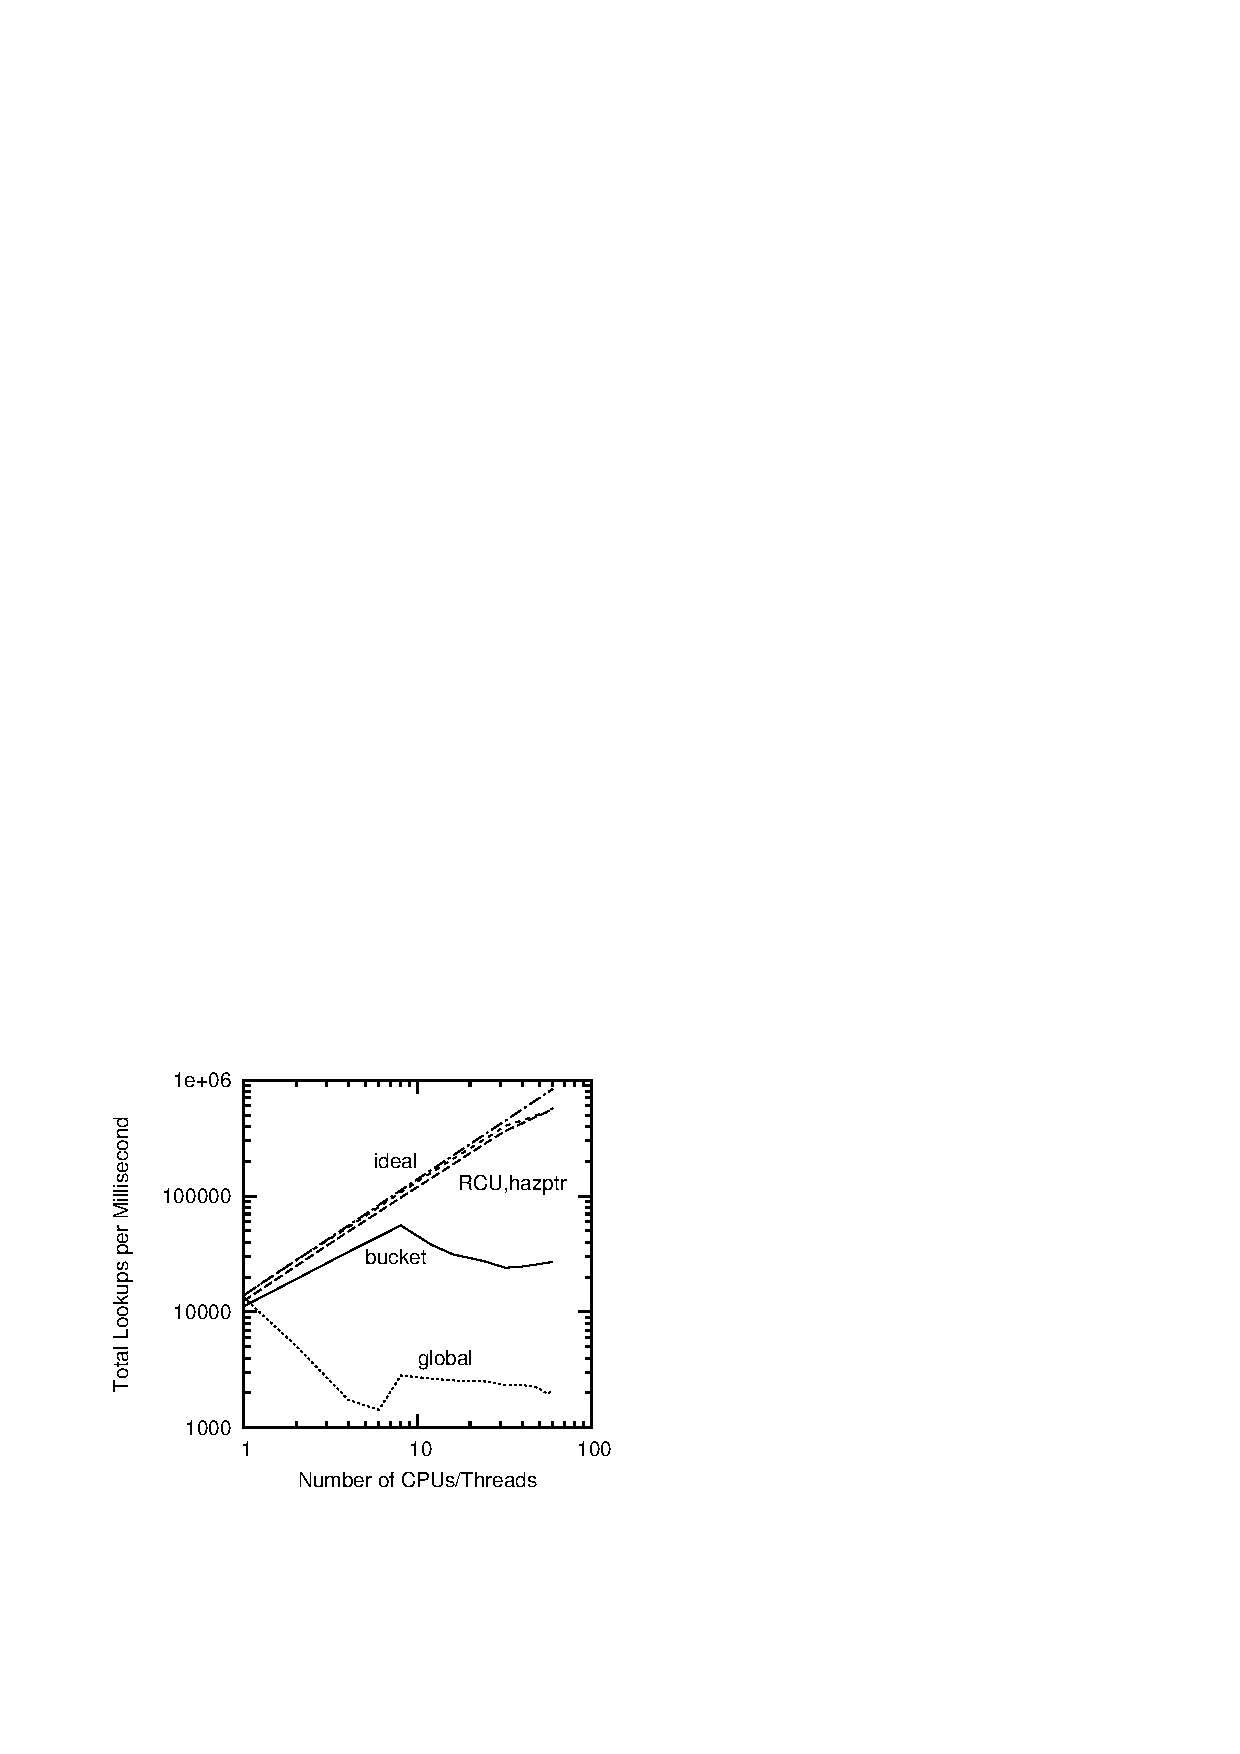
\includegraphics{datastruct/zoocpu}}
\end{center}
\caption{Read-Only RCU-Protected Hash-Table Performance For Schr\"odinger's Zoo}
\label{fig:datastruct:Read-Only RCU-Protected Hash-Table Performance For Schroedinger's Zoo}
\end{figure}

Figure~\ref{fig:datastruct:Read-Only RCU-Protected Hash-Table Performance For Schroedinger's Zoo}
shows the read-only performance of RCU-protected and hazard-pointer-protected
hash tables against the previous section's per-bucket-locked implementation.
As you can see, both RCU and hazard pointers achieve near-ideal performance
and scalability despite the larger numbers of threads and the NUMA effects.
Results from a globally locked implementation are also shown, and as expected
the results are even worse than those of the per-bucket-locked implementation.
RCU does slightly better than hazard pointers, but the difference is not
readily visible in this log-scale plot.

\begin{figure}[tb]
\begin{center}
\resizebox{3in}{!}{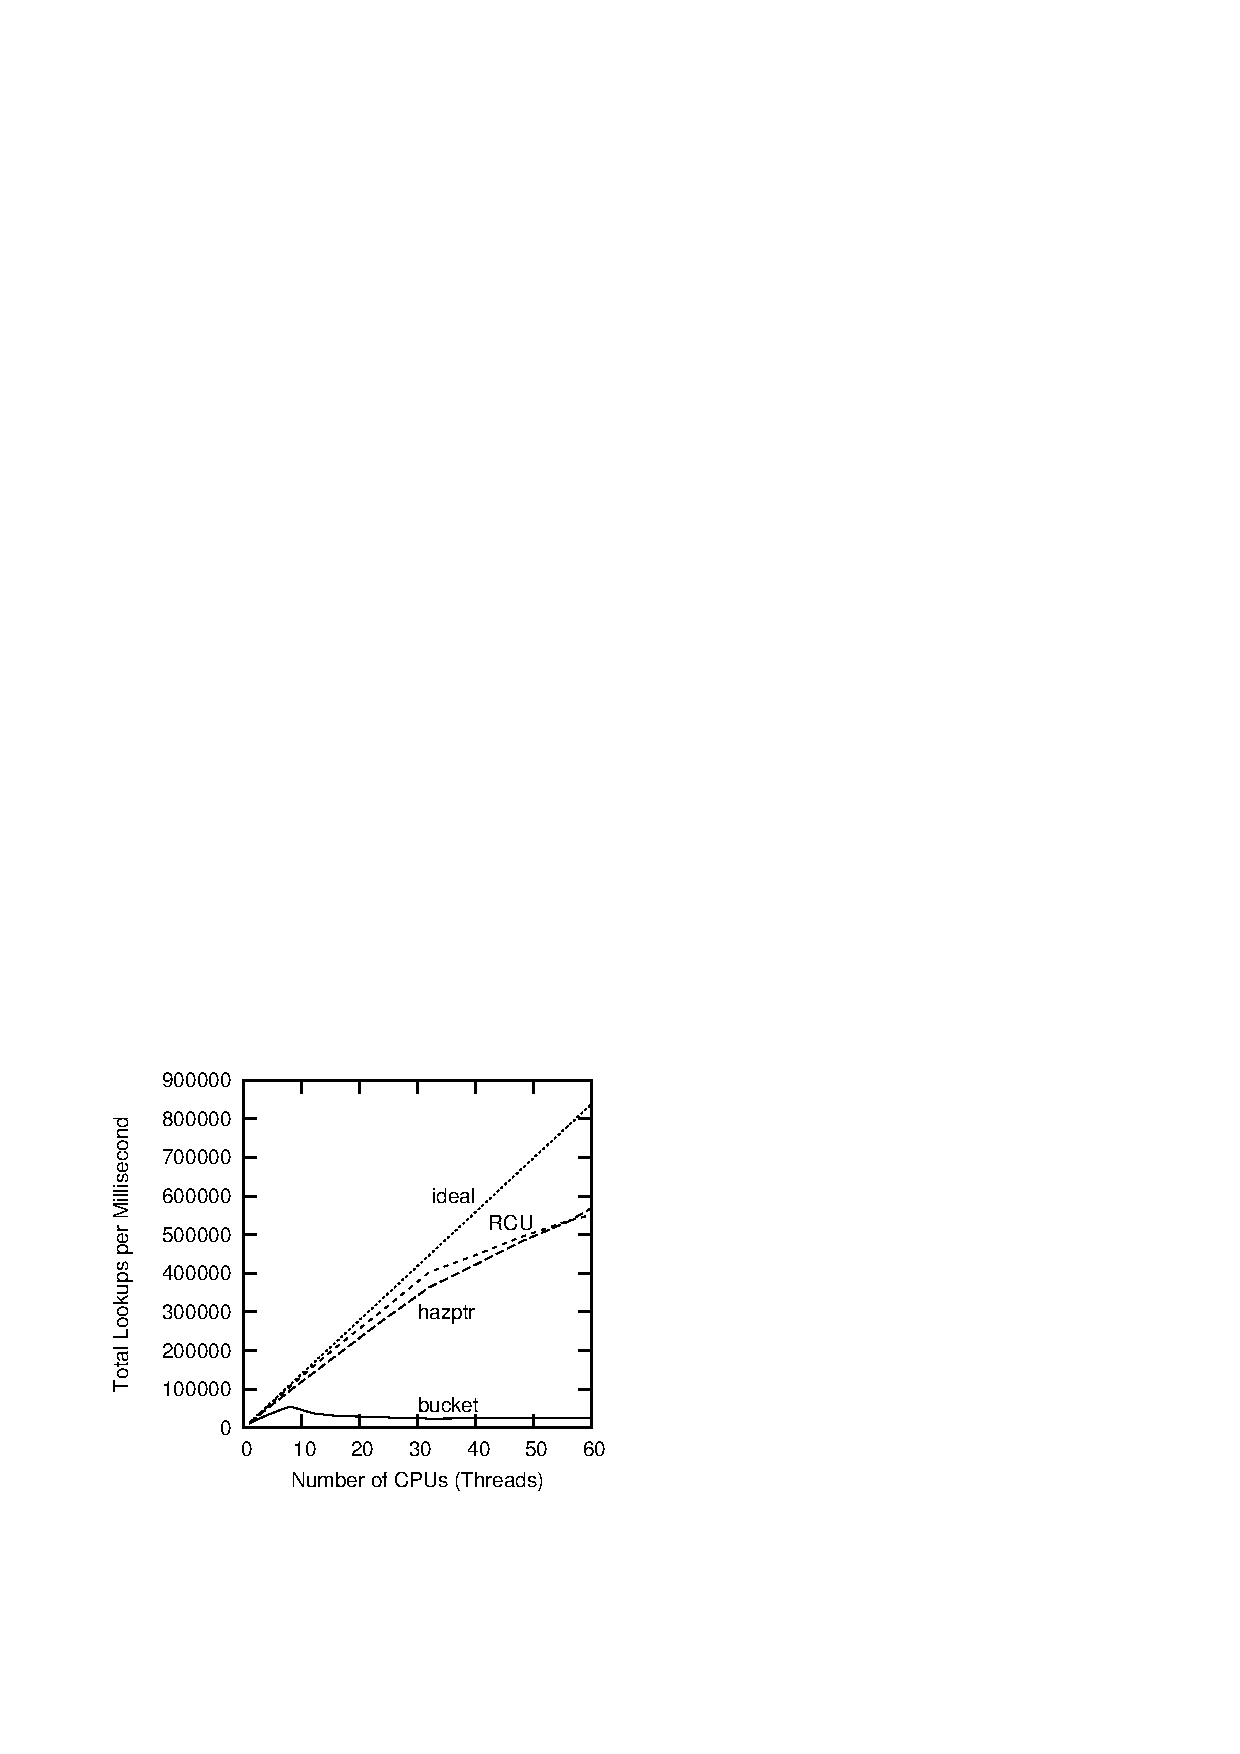
\includegraphics{datastruct/zoocpulin}}
\end{center}
\caption{Read-Only RCU-Protected Hash-Table Performance For Schr\"odinger's Zoo, Linear Scale}
\label{fig:datastruct:Read-Only RCU-Protected Hash-Table Performance For Schroedinger's Zoo, Linear Scale}
\end{figure}

Figure~\ref{fig:datastruct:Read-Only RCU-Protected Hash-Table Performance For Schroedinger's Zoo, Linear Scale}
shows the same data on a linear scale.
This drops the global-locking trace into the x-axis, but allows the
relative performance of RCU and hazard pointers to be more readily
discerned.
Both show a change in slope at 32 CPUs, and this is due to hardware
multithreading.
At 32 and fewer CPUs, each thread has a core to itself.
In this regime, RCU does better than does hazard pointers because
hazard pointers's read-side memory barriers result in dead time within
the core.
In short, RCU is better able to utilize a core from a single hardware
thread than is hazard pointers.

This situation changes above 32 CPUs.
Because RCU is using more than half of each core's resources from a
single hardware thread, RCU gains relatively litte benefit from the
second hardware thread in each core.
The slope of hazard pointers's trace also decreases at 32 CPUs, but
less dramatically.
This is because the second hardware thread is able to fill in the time
that the first hardware thread is stalled due to memory-barrier latency.
As we will see in later sections, hazard pointers's second-hardware-thread
advantage depends on the workload.

\begin{figure}[tb]
\begin{center}
\resizebox{3in}{!}{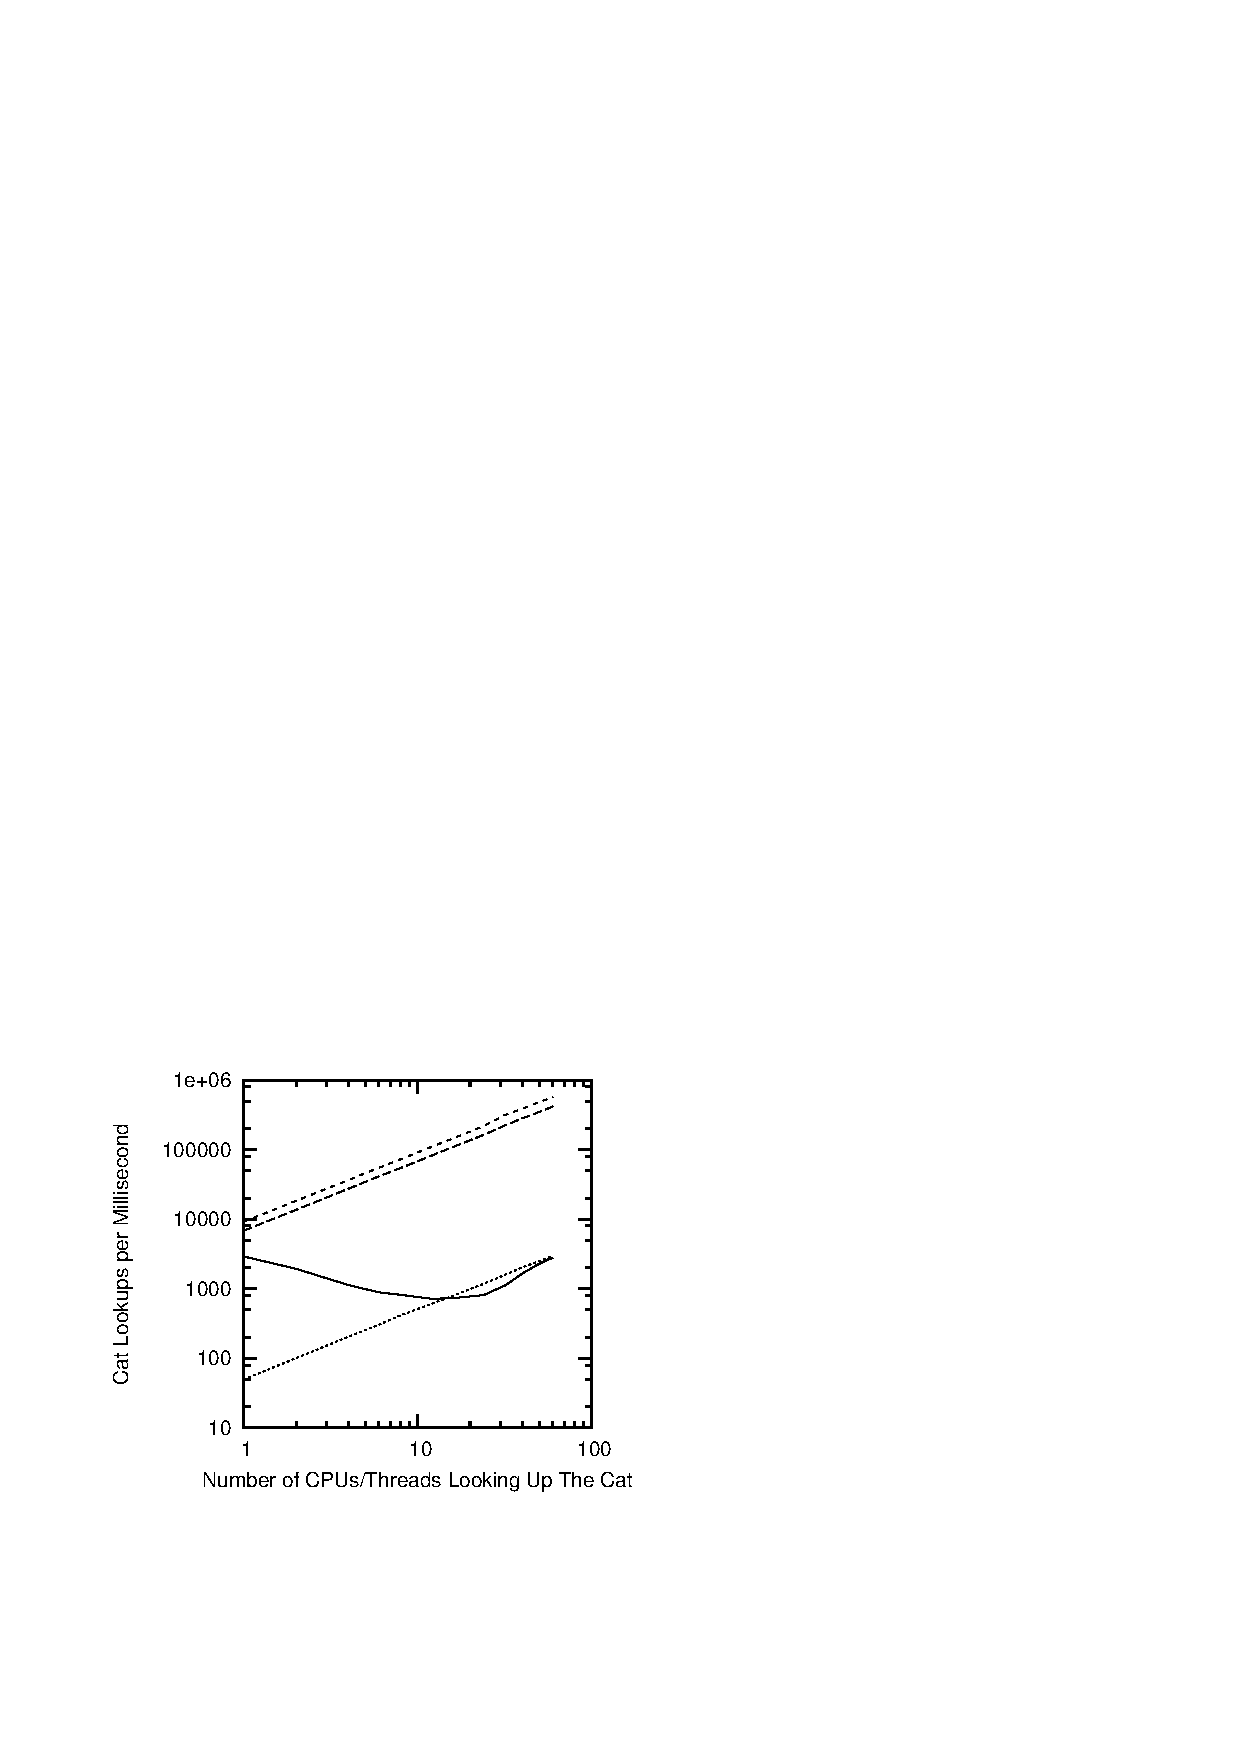
\includegraphics{datastruct/zoocatonly}}
\end{center}
\caption{Read-Side Cat-Only RCU-Protected Hash-Table Performance For Schr\"odinger's Zoo at 60 CPUs}
\label{fig:datastruct:Read-Side Cat-Only RCU-Protected Hash-Table Performance For Schroedinger's Zoo at 60 CPUs}
\end{figure}

Schr\"odinger is constantly surprised by the popularity of his
cat~\cite{ErwinSchroedinger1935Cat}, but recognizes the need to reflect
this in his design.
Figure~\ref{fig:datastruct:Read-Side Cat-Only RCU-Protected Hash-Table Performance For Schroedinger's Zoo at 60 CPUs}
shows the results of 60-CPU runs, varying the number of CPUs that are
doing nothing but looking up the cat.
Both RCU and hazard pointers respond well to this challenge, but
bucket locking scales negatively, eventually performing even worse
than global locking.
This should not be a surprise because if all CPUs are doing nothing
but looking up the cat, the lock corresponding to the cat's bucket
is for all intents and purposes a global lock.

This cat-only benchmark illustrates one potential problem with
sharding approaches that fully partition the database.
Given these approaches, only the CPUs associated with the cat's
partition would be able to access the cat, limiting the cat-only
throughput.
Nevertheless, a great many applications have better load-spreading
properties, and for these applications full partitioning works
quite well.

\begin{figure}[tb]
\begin{center}
\resizebox{3in}{!}{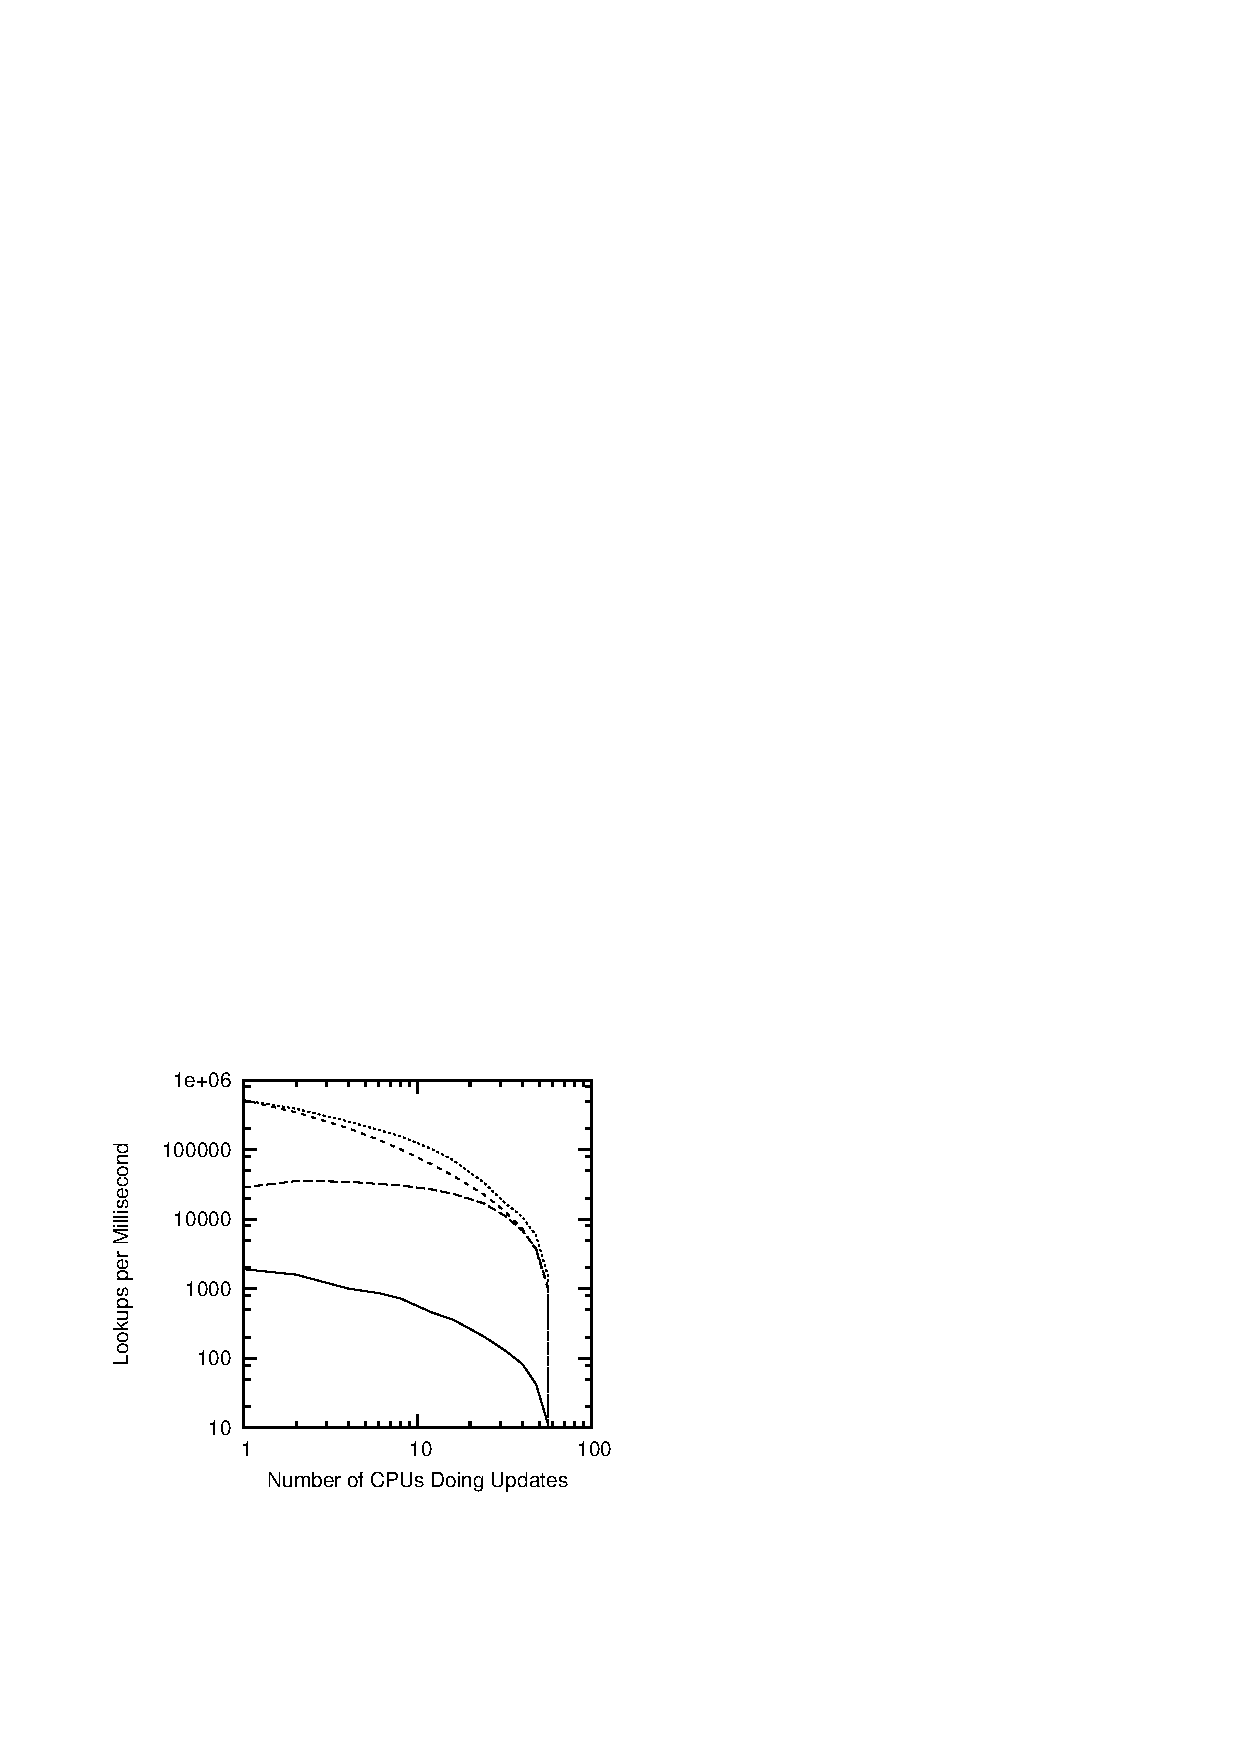
\includegraphics{datastruct/zooupdatelu}}
\end{center}
\caption{Read-Side RCU-Protected Hash-Table Performance For Schr\"odinger's Zoo at 60 CPUs}
\label{fig:datastruct:Read-Side RCU-Protected Hash-Table Performance For Schroedinger's Zoo at 60 CPUs}
\end{figure}

Of course, if we were only ever going to read the data, we would not need
any concurrency control to begin with.
Figure~\ref{fig:datastruct:Read-Side RCU-Protected Hash-Table Performance For Schroedinger's Zoo at 60 CPUs}
therefore shows the effect on lookups of increasing numbers of updating
CPUs.
At the extreme left-hand side of this graph, all 60 CPUs are doing lookups,
while to the right all 60 CPUs are doing updates.
For all four implementations, the number of lookups per millisecond
decreases as the number of updating CPUs increases, of course reaching
zero updates per millisecond when all 60 CPUs are updating.
RCU does well relative to hazard pointers due to the fact that hazard
pointers's read-side memory barriers incur greater overhead in the
presence of updates.
This situation indicates that hardware heavily optimizes memory-barrier
execution in the read-only case.

\begin{figure}[tb]
\begin{center}
\resizebox{3in}{!}{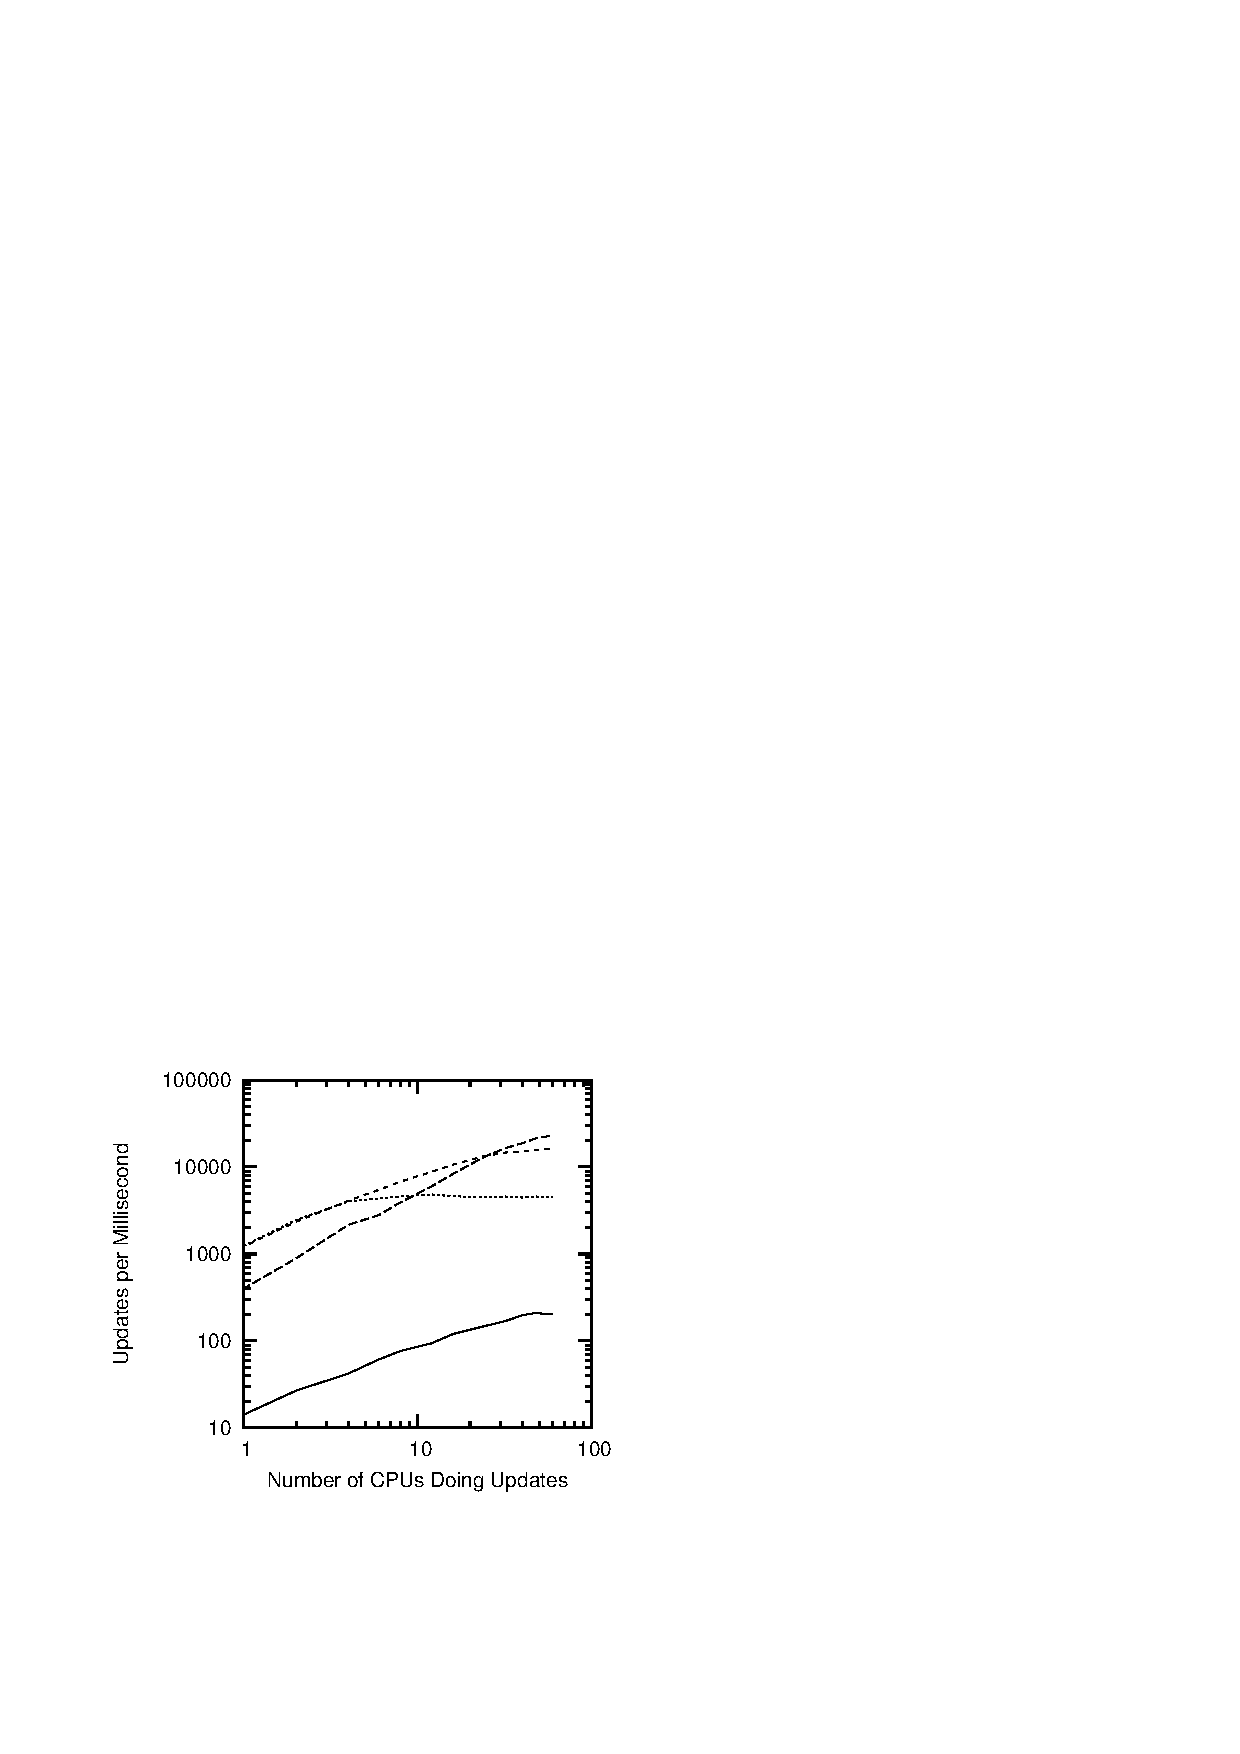
\includegraphics{datastruct/zooupdate}}
\end{center}
\caption{Update-Side RCU-Protected Hash-Table Performance For Schr\"odinger's Zoo at 60 CPUs}
\label{fig:datastruct:Update-Side RCU-Protected Hash-Table Performance For Schroedinger's Zoo at 60 CPUs}
\end{figure}

Figure~\ref{fig:datastruct:Update-Side RCU-Protected Hash-Table Performance For Schroedinger's Zoo at 60 CPUs}
shows how updates vary as more of the 60 CPUs are doing updates.
Hazard pointers and RCU start off with a significant advantage because,
unlike bucket locking, readers do not exclude updaters.
However, as the number of updating CPUs increases, the increased update-side
overhead starts to make its presence knowsn, first for RCU and next for
hazard pointers.
Of course, all three of these implementations fare much better than does
global locking.

However, it is quite possible that the differences in lookup performance
in the presence of updates is affected by the differences in update
rates.
One way to check this is to artificially throttle the update rates of
per-bucket locking and hazard pointers to match that of RCU.
Doing so does not significantly improve the lookup performace of
per-bucket locking, nor does it close the gap between hazard pointers
and RCU.
However, removing hazard pointers's read-side memory barriers
(thus resulting in an unsafe implementation of hazard pointers)
does nearly close the gap between hazard pointers and RCU.
The resulting unsafe implementation of hazard pointers will nevertheless
usually be reliable enough for benchmarking purposes.

\QuickQuiz{}
	The dangers of extrapolating from eight CPUs to 60 CPUs was
	made quite clear in
	Section~\ref{sec:datastruct:Hash-Table Performance}.
	But why should extrapolating up from 60 CPUs be any safer?
\QuickQuizAnswer{
	It isn't any safer, and a useful exercise would be to run these
	programs on larger systems.
	That said, other testing has shown that RCU read-side primitives
	offer consistent performance and scalability up to at least 1024 CPUs.
} \QuickQuizEnd

\subsection{RCU-Protected Hash Table Discussion}
\label{sec:datastruct:RCU-Protected Hash Table Discussion}

One consequence of the RCU and hazard-pointer implementations is
that a pair of concurrent readers might disagree on the state of
the cat.
For example, one of the readers might have fetched the pointer to
the cat's data structure just before it was removed, while another
reader might have fetched this same pointer just afterwards.
The first reader would then believe that the cat was alive, while
the second reader would believe that the cat was dead.

Of course, this situation is completely fitting for Schr\"odinger's
cat, but it turns out that it is quite reasonable for normal
non-quantum cats as well.

The reason for this is that it is impossible to determine exactly
when an animal is born or dies.

To see this, let's suppose that we detect a cat's death by heartbeat.
This raise the question of exactly how long we should wait after the
last heartbeat before declaring death.
It is clearly ridiculous to wait only one millisecond, because then
a healthy living cat would have to be declared dead---and then
resurrected---more than once every second.
It is equally ridiculous to wait a full month, because by that time
the poor cat's death would have made itself very clearly known
via olfactory means.

\begin{figure}[htb]
\begin{center}
\resizebox{3in}{!}{
\includegraphics{cartoons/2013-08-is-it-dead}}
\end{center}
\caption{Even Veterinarians Disagree!}
\ContributedBy{Figure}{fig:datastruct:Even Veterinarians Disagree}{Melissa McKenney}
\end{figure}

Because an animal's heart can stop for some seconds and then start up
again, there is a tradeoff between timely recognition of death and
probability of false alarms.
It is quite possible that a pair of veterinarians might disagree on
the time to wait between the last heartbeat and the declaration of
death.
For example, one veterinarian might declare death thirty seconds after
the last heartbeat, while another might insist on waiting a full
minute.
In this case, the two veterinarians would disagree on the state of the
cat for the second period of thirty seconds following the last heartbeat,
as fancifully depicted in
Figure~\ref{fig:datastruct:Even Veterinarians Disagree}.

Of course, Heisenberg taught us to live with this sort of
uncertainty~\cite{WeinerHeisenberg1927Uncertain}, which is a good
thing because computing hardware and software acts similarly.
For example, how do you know that a piece of computing hardware
has failed?
Often because it does not respond in a timely fashion.
Just like the cat's heartbeat, this results in a window of
uncertainty as to whether or not the hardware has failed.

Furthermore, most computing systems are intended to interact with
the outside world.
Consistency with the outside world is therefore of paramount importance.
However, as we saw in
Figure~\ref{fig:defer:Response Time of RCU vs. Reader-Writer Locking},
increased internal consistency can come at the expense of external
consistency.
Techniques such as RCU and hazard pointers give up some degree of
internal consistency to attain improved external consistency.

In short, internal consistency is not a natural part of all problem domains,
and often come at great expense, either in terms of performance
and scalability or in terms of external consistency.

\section{Non-Partitionable Data Structures}
\label{sec:datastruct:Non-Partitionable Data Structures}

Hash tables are perfectly partitionable, but only if they are of fixed
size.
However, it turns out that it is possible to construct high-performance
scalable RCU-protected hash tables, as described in the following sections.

\subsection{Resizable Hash Table Design}
\label{sec:datastruct:Resizable Hash Table Design}

In happy contrast to the situation in the early 2000s, there are now
no fewer than three different types of scalable RCU-protected hash
tables.
The first (and simplest) was developed for the Linux kernel by
Herbert Xu~\cite{HerbertXu2010RCUResizeHash}, and is described in the
following sections.
The other two are covered briefly in
Section~\ref{sec:datastruct:Other Resizable Hash Tables}.

The key insight behind the first hash-table implementation is that
each data element can have two sets of list pointers, with one set
currently being used by RCU readers (as well as by non-RCU updaters)
and the other being used to construct a new resized hash table.
This approach allows lookups, insertions, and deletions to run
concurrently with a resize operation.

\begin{figure}[tb]
\begin{center}
\resizebox{3in}{!}{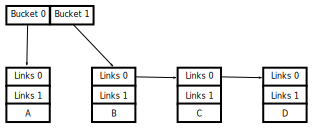
\includegraphics{datastruct/hashxu-a}}
\end{center}
\caption{Growing a Double-List Hash Table, State (a)}
\label{fig:datastruct:Growing a Double-List Hash Table, State (a)}
\end{figure}

\begin{figure}[tb]
\begin{center}
\resizebox{3in}{!}{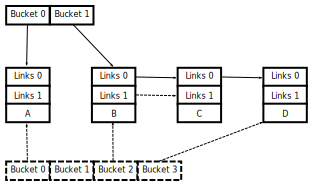
\includegraphics{datastruct/hashxu-b}}
\end{center}
\caption{Growing a Double-List Hash Table, State (b)}
\label{fig:datastruct:Growing a Double-List Hash Table, State (b)}
\end{figure}

The resize operation proceeds as shown in
Figures~\ref{fig:datastruct:Growing a Double-List Hash Table, State (a)}-\ref{fig:datastruct:Growing a Double-List Hash Table, State (d)},
with initial two-bucket state~(a) and with time advancing from top to bottom.
The initial state uses the zero-index links to chain the elements into
hash buckets.
A four-bucket array is allocated, and the one-index links are used to
chain the elements into these four new hash buckets.
This results in state~(b) shown in
Figure~\ref{fig:datastruct:Growing a Double-List Hash Table, State (b)},
with readers still using the original two-bucket array.

\begin{figure}[tb]
\begin{center}
\resizebox{3in}{!}{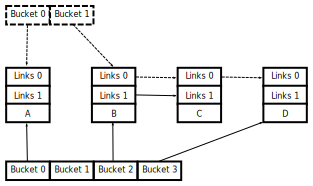
\includegraphics{datastruct/hashxu-c}}
\end{center}
\caption{Growing a Double-List Hash Table, State (c)}
\label{fig:datastruct:Growing a Double-List Hash Table, State (c)}
\end{figure}

\begin{figure}[tb]
\begin{center}
\resizebox{3in}{!}{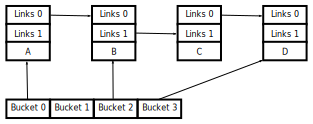
\includegraphics{datastruct/hashxu-d}}
\end{center}
\caption{Growing a Double-List Hash Table, State (d)}
\label{fig:datastruct:Growing a Double-List Hash Table, State (d)}
\end{figure}

The new four-bucket array is exposed to readers and then a grace-period
operation waits for all readers, resulting in state~(c), shown in
Figure~\ref{fig:datastruct:Growing a Double-List Hash Table, State (c)}.
In this state, all readers are using the new four-bucket array,
which means that the old two-bucket array may now be freed, resulting
in state~(d), shown in
Figure~\ref{fig:datastruct:Growing a Double-List Hash Table, State (d)}.

This design leads to a relatively straightforward implementation,
which is the subject of the next section.

\subsection{Resizable Hash Table Implementation}
\label{sec:datastruct:Resizable Hash Table Implementation}

\begin{figure}[tb]
{ \scriptsize
\begin{verbatim}
 1 struct ht_elem {
 2   struct rcu_head rh;
 3   struct cds_list_head hte_next[2];
 4   unsigned long hte_hash;
 5 };
 6 
 7 struct ht_bucket {
 8   struct cds_list_head htb_head;
 9   spinlock_t htb_lock;
10 };
11 
12 struct ht {
13   long ht_nbuckets;
14   long ht_resize_cur;
15   struct ht *ht_new;
16   int ht_idx;
17   void *ht_hash_private;
18   int (*ht_cmp)(void *hash_private,
19                 struct ht_elem *htep,
20                 void *key);
21   long (*ht_gethash)(void *hash_private,
22                      void *key);
23   void *(*ht_getkey)(struct ht_elem *htep);
24   struct ht_bucket ht_bkt[0];
25 };
26 
27 struct hashtab {
28   struct ht *ht_cur;
29   spinlock_t ht_lock;
30 };
\end{verbatim}
}
\caption{Resizable Hash-Table Data Structures}
\label{fig:datastruct:Resizable Hash-Table Data Structures}
\end{figure}

Resizing is accomplished by the classic approach of inserting a level
of indirection, in this case, the \co{ht} structure shown on
lines~12-25 of
Figure~\ref{fig:datastruct:Resizable Hash-Table Data Structures}.
The \co{hashtab} structure shown on lines~27-30 contains only a
pointer to the current \co{ht} structure along with a spinlock that
is used to serialize concurrent attempts to resize the hash table.

The \co{ht} structure represents a specific size of the hash table,
as specified by the \co{->ht_nbuckets} field on line~13.
The size is stored in the same structure containing the array of
buckets (\co{->ht_bkt[]} on line~24) in order to avoid mismatches between
the size and the array.
The \co{->ht_resize_cur} field on line~14 is equal to -1 unless a resize
operation
is in progress, in which case it indicates the index of the bucket whose
elements are being inserted into the new hash table, which is referenced
by the \co{->ht_new} field on line~15.
If there is no resize operation in progress, \co{->ht_new} is \co{NULL}.
Thus, a resize operation proceeds by allocating a new \co{ht} structure
and referencing it via the \co{->ht_new} pointer, then advancing
\co{->ht_resize_cur} through the old table's buckets.
When all the elements have been added to the new table, the new
table is linked into the \co{hashtab} structure's \co{->ht_cur} field.
Once all old readers have completed, the old hash table's \co{ht} structure
may be freed.

The \co{->ht_idx} field on line~16 indicates which of the two sets of
list pointers are being used by this instantiation of the hash table,
and is used to index the \co{->hte_next[]} array in the \co{ht_bucket}
structure on line~3.

The \co{->ht_hash_private}, \co{->ht_cmp()}, \co{->ht_gethash()},
and \co{->ht_getkey()} fields collectively define the per-element
key and the hash function.
The \co{->ht_hash_private} allows the hash function to be
perturbed~\cite{McKenney89c,McKenney90,McKenney91}, which can be
used to avoid denial-of-service attacks based on statistical
estimation of the parameters used in the hash function.
The \co{->ht_cmp()} function compares a specified key with that of
the specified element,
the \co{->ht_gethash()} calculates the specified key's hash,
and \co{->ht_getkey()} extracts the key from the enclosing data
element.

The \co{ht_bucket} structure is the same as before, and the
\co{ht_elem} structure differs from that of previous implementations
only in providing a two-element array of list pointer sets in place of
the prior single set of list pointers.

\begin{figure}[tb]
{ \scriptsize
\begin{verbatim}
 1 void hashtab_lock_mod(struct hashtab *htp_master,
 2                       void *key)
 3 {
 4   long b;
 5   struct ht *htp;
 6   struct ht_bucket *htbp;
 7   struct ht_bucket *htbp_new;
 8 
 9   rcu_read_lock();
10   htp = rcu_dereference(htp_master->ht_cur);
11   htbp = ht_get_bucket_single(htp, key, &b);
12   spin_lock(&htbp->htb_lock);
13   if (b > htp->ht_resize_cur)
14     return;
15   htp = htp->ht_new;
16   htbp_new = ht_get_bucket_single(htp, key, &b);
17   spin_lock(&htbp_new->htb_lock);
18   spin_unlock(&htbp->htb_lock);
19 }
20 
21 void hashtab_unlock_mod(struct hashtab *htp_master,
22                         void *key)
23 {
24   long b;
25   struct ht *htp;
26   struct ht_bucket *htbp;
27 
28   htp = rcu_dereference(htp_master->ht_cur);
29   htbp = ht_get_bucket(&htp, key, &b, NULL);
30   spin_unlock(&htbp->htb_lock);
31   rcu_read_unlock();
32 }
\end{verbatim}
}
\caption{Resizable Hash-Table Update-Side Concurrency Control}
\label{fig:datastruct:Resizable Hash-Table Update-Side Concurrency Control}
\end{figure}

Read-side concurrency control is provided by RCU as was shown in
Figure~\ref{fig:datastruct:RCU-Protected Hash-Table Read-Side Concurrency Control},
but update-side concurrency must now deal with the possibility of a
concurrent resize operation as shown in
Figure~\ref{fig:datastruct:Resizable Hash-Table Update-Side Concurrency Control}.

\subsection{Resizable Hash Table Discussion}
\label{sec:datastruct:Resizable Hash Table Discussion}

@@@ Resizable hash tables.

\subsection{Other Resizable Hash Tables}
\label{sec:datastruct:Other Resizable Hash Tables}

One shortcoming of the resizable hash table described earlier in this
section is memory consumption.
Each data element has two pairs of linked-list pointers rather than just
one.
Is it possible to create an RCU-protected resizable hash table that
makes do with just one pair?

It turns out that the answer is ``yes.''
Josh Triplett et al.~\cite{Triplett:2011:RPHash}
produced a \emph{relativistic hash table} that incrementally
splits and combines corresponding hash chains so that readers always
see valid hash chains at all points during the resizing operation.
This incremental splitting and combining relies on the fact that it
is harmless for a reader to see a data element that should be in some
other hash chain: When this happens, the reader will simply ignore the
extraneous data element due to key mismatches.

\begin{figure}[tb]
\begin{center}
\resizebox{3in}{!}{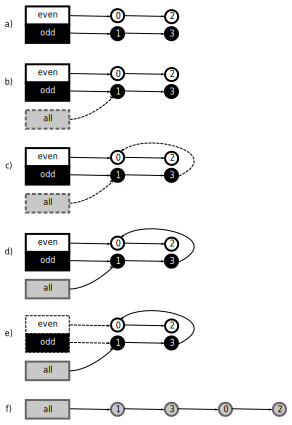
\includegraphics{datastruct/zipperhashshrink}}
\end{center}
\caption{Shrinking a Relativistic Hash Table}
\label{fig:datastruct:Shrinking a Relativistic Hash Table}
\end{figure}

The process of shrinking a relativistic hash table by a factor of two
is shown in
Figure~\ref{fig:datastruct:Shrinking a Relativistic Hash Table},
in this case shrinking a two-bucket hash table into a one-bucket
hash table, otherwise known as a linear list.
This process works by coalescing pairs of buckets in the old larger hash
table into single buckets in the new smaller hash table.
For this process to work correctly, we clearly need to constrain the hash
functions for the two tables.
One such constraint is to use the same underlying hash function for
both tables, but to throw out the low-order bit when shrinking from
large to small.
For example, the old two-bucket hash table would
use the two top bits of the value, while the new one-bucket hash table
could use the top bit of the value.
In this way, a given pair of adjacent even and odd buckets in the old
large hash table can be coalesced into a single bucket in the new small
hash table, while still having a single hash value cover all of the
elements in that single bucket.

The initial state is shown at the top of the figure, with time advancing
from top to bottom.
The shrinking process begins by allocating the new smaller array of
buckets, and having each bucket of this new smaller array reference
the first element of one of the buckets of the corresponding pair in
the old large hash table, resulting in state~(b).

Then the two hash chains are linked together, resulting in state~(c).
In this state, readers looking up an even-numbered element see no change,
and readers looking up elements~1 and~3 likewise see no change.
However, readers looking up some other odd number will also traverse
elements~0 and~2.
This is harmless because any odd number will compare not-equal to these
two elements.
There is some performance loss, but on the other hand, this is exactly
the same performance loss that will be experienced once the new small
hash table is fully in place.

Next, the new small hash table is made accessible to readers, resulting
in state~(d).
Note that older readers might still be traversing the old large hash
table, so in this state both hash tables are in use.

The next step is to wait for all pre-existing readers to complete,
resulting in state~(e).
In this state, all readers are using the new small hash table, so that
the old large hash table's buckets may be freed, resulting in the final
state~(f).

\begin{figure}[tb]
\begin{center}
\resizebox{3in}{!}{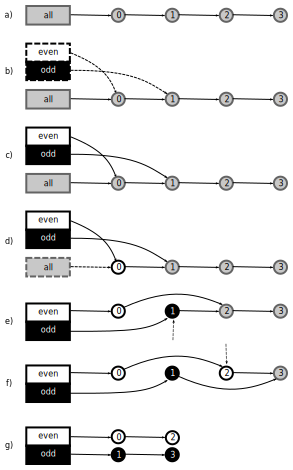
\includegraphics{datastruct/zipperhashgrow}}
\end{center}
\caption{Growing a Relativistic Hash Table}
\label{fig:datastruct:Growing a Relativistic Hash Table}
\end{figure}

Growing a relativistic hash table reverses the shrinking process,
but requires more grace-period steps, as show in
Figure~\ref{fig:datastruct:Growing a Relativistic Hash Table}.
The initial state~(a) is at the top of this figure, with time advancing
from top to bottom.

We start by allocating the new large two-bucket hash table, resulting
in state~(b).
Note that each of these new buckets references the first element destined
for that bucket.
These new buckets are published to readers, resulting in state~(c).
After a grace-period operation, all readers are using the new large
hash table, resulting in state~(d).
In this state, only those readers traversing the even-values hash bucket
traverse element~0, which is therefore now colored white.

At this point, the old small hash buckets may be freed, although many
implementations use these old buckets to track progress ``unzipping''
the list of items into their respective new buckets.
The last even-numbered element in the first consecutive run of such
elements now has its pointer-to-next updated to reference the following
even-numbered element.
After a subsequent grace-period operation, the result is state~(e).
The vertical arrow indicates the next element to be unzipped, and
element~1 is now colored black to indicate that only those readers traversing
the odd-values hash bucket may reach it.

Next, the last odd-numbered element in the first consecutive run of such
elements now has its pointer-to-next updated to reference the following
odd-numbered element.
After a subsequent grace-period operation, the result is state~(f).
A final unzipping operation (including a grace-period operation)
results in the final state~(g).

In short, the relativistic hash table reduces the number of per-element
list pointers at the expense of additional grace periods incurred during
resizing.
These additional grace periods are usually not a problem because
insertions, deletions, and lookups may proceed concurrently with
a resize operation.

It turns out that it is possible to reduce the per-element memory overhead
from a pair of pointers to a single pointer, while still retaining
$O(1)$ deletions.
This is accomplished by augmenting split-order
list~\cite{OriShalev2006SplitOrderListHash}
with RCU
protection~\cite{MathieuDesnoyers2009URCU,PaulMcKenney2013LWNURCUhash}.
The data elements in the hash table are arranged into a single
sorted linked list, with each hash bucket referencing the first element
in that bucket.
Elements are deleted by setting low-order bits in their pointer-to-next
fields, and these elements are removed from the list by later traversals
that encounter them.

This RCU-protected split-order list is complex, but offers lock-free
progress guarantees for all insertion, deletion, and lookup operations.
Such guarantees can be important in real-time applications.
An implementation is available from recent versions of the userspace RCU
library~\cite{MathieuDesnoyers2009URCU}.

\section{Other Data Structures}
\label{sec:datastruct:Other Data Structures}

The preceding sections have focused on data structures that enhance
concurrency due to partitionability
(Section~\ref{sec:datastruct:Partitionable Data Structures}),
efficient handling of read-mostly access patterns
(Section~\ref{sec:datastruct:Read-Mostly Data Structures}),
or application of read-mostly techniques to avoid
non-partitionability
(Section~\ref{sec:datastruct:Non-Partitionable Data Structures}).
This section gives a brief review of other data structures.

One of the hash table's greatest advantages for parallel use is that it
is fully partitionable, at least while not being resized.
One way of preserving the partitionability and the size independence is
to use a radix tree, which is also called a trie.
Tries partition the search key, using each successive key partition
to traverse the next level of the trie.
As such, a trie can be thought of as a set of nested hash tables,
thus providing the required partitionability.
One disadvantage of tries is that a sparse key space can result in
inefficient use of memory.
There are a number of compression techniques that may be used to
work around this disadvantage, including hashing the key value to
a smaller keyspace before the
traversal~\cite{RobertOlsson2006a}.
Radix trees are heavily used in practice, including in the Linux
kernel~\cite{NickPiggin2006radixtree}.

One important special case of both a hash table and a trie is what is
perhaps the oldest of data structures, the array and its multi-dimensional
counterpart, the matrix.
The fully partitionable nature of matrices is exploited heavily in
concurrent numerical algorithms.

Self-balancing trees are heavily used in sequential code, with
AVL trees and red-black trees being perhaps the most well-known
examples~\cite{ThomasHCorman2001Algorithms}.
Early attempts to parallelize AVL trees were complex and not necessarily
all that efficient~\cite{Ellis80},
however, more recent work on red-black trees provides better
performance and scalability by using RCU for readers and hashed arrays
of locks\footnote{
	In the guise of swissTM~\cite{AleksandarDragovejic2011STMnotToy},
	which is a variant of software transactional memory in which
	the developer flags non-shared accesses.}
to protect reads and updates,
respectively~\cite{PhilHoward2011RCUTMRBTree,PhilipWHoward2013RCUrbtree}.
It turns out that red-black trees rebalance aggressively, which works
well for sequential programs, but not necessarily so well for parallel
use.
Recent work has therefore made use of RCU-protected ``bonsai trees''
that rebalance less aggressively~\cite{AustinClements2012RCULinux:mmapsem},
trading off optimal tree depth to gain more efficient concurrent updates.

Concurrent skip lists lend themselves well to RCU readers, and in fact
represents an early academic use of a technique resembling
RCU~\cite{Pugh90}.

Concurrent double-ended queues were discussed in
Section~\ref{sec:SMPdesign:Double-Ended Queue},
and concurrent stacks and queues have a long history~\cite{Treiber86},
though not normally the most impressive performance or scalability.
They are nevertheless a common feature of concurrent
libraries~\cite{PaulMcKenney2013LWNURCUqueuestack}.
Researchers have recently proposed relaxing the ordering constraints
of stacks and queues~\cite{Shavit:2011:DSM:1897852.1897873},
with some work indicating that relaxed-ordered queues actually have
better ordering properties than do strict FIFO
queues~\cite{AndreasHaas2012FIFOisnt,ChristophMKirsch2012FIFOisntTR,AndreasHaas2013CFRelaxedQueues}.

It seems likely that continued work with concurrent data structures will
produce novel algorithms with surprising properties.

\section{Micro-Optimization}
\label{sec:datastruct:Micro-Optimization}

\subsection{Specialization}
\label{sec:datastruct:Specialization}

% @@@ hash table that has unsigned long for key.  Compare performance
% to the RCU-protected hash tables with general keys.

\subsection{Bits and Bytes}
\label{sec:datastruct:Bits and Bytes}

Bit fields, endianness, packing.

\subsection{Hardware Considerations}
\label{sec:datastruct:Hardware Considerations}

CPU word alignment, cache alignment.

\emph{@@@ pull in material from Orran Kreiger's 1995 paper (permission
granted).}

\section{Summary}
\label{sec:datastruct:Summary}

